\documentclass[class=report]{standalone}
\usepackage{pacco}
\begin{document}
	\chapter{A first study in stochastic processes: Martingales}
	Okay, I'll admit that this part is really hard for me to follow. I am already broken down by Professor Polito's lectures and right now... I only want to be happy again. Please note that the astonishing drop in the quality of the notes is not my fault. This shit should be easier to explain but they manage to mess this up anyway. 
	\section{Revising stochastic processes and filtrations}
	\begin{notation}
		\begin{enumerate}
			\item we will work in a fixed probability space $(\Omega,\HS,\pr)$;
			\item we will denote an index set $\T$ (which is usually interpreted as time). It could be $\T=\N$ or $\T=\R$, for example;
			\item $\{X_t:t\in \T\}$ is a \rv{} taking values in the product space
			\[(F,\F)=(E^{\T},\E^\T).\]
			We can think of this as an evolving stochastic process.
		\end{enumerate}
	\end{notation}
	Let $\T$ be a subset of $\R$. For each $t\in\T$ let $\F_t$ be a sub-\sa{} of $\HS$. The family $\F=\left\{\F_t:t\in\T\right\}$ is called a \emph{filtration} provided that
	\[\F_s\in\F_t\qquad\every s<t.\]
	\begin{definition}
		A \emph{stochastic process} $X={(X_t)}_{t\in\T}$ generates a filtration that is named \emph{natural filtration}.
	\end{definition}
	As the time passes, I discover more and more information about $\HS$. Each process defines a filtration by generating a ``flow of information''.
	\begin{example}
		Imagine a car competition composed by two different races. Consider the events
		\[\begin{array}{l}
			\omega=\left\{\text{car $A$ wins}\right\}\\
			\ell=\left\{\text{car $A$ loses}\right\}.
		\end{array}\]
		Consider 2 races: our $\Omega$ will be
		\[\Omega=\left\{\omega\omega,\ell\omega,\omega\ell,\ell\ell\right\}.\]
		Before the starting of the race, at time 0, we have no information about what is going to happen so our filtration will be
		\[\F_0=\left\{\underbracket{\left\{0\right\}}_{\emptyset},\underbracket{\left\{\omega\omega,\ell\omega,\omega\ell,\ell\ell\right\}}_{\Omega}\right\}\]
		which is the trivial \sa{}. Remember that in this case the empty set $\emptyset$ represents impossible events (e.g. all cars win all races). So the \rv{} $X_0$ measurable with respect to $\F_0$ maps all the outcomes of the race to the same value. The idea is that we cannot ask ourselves ``what is the probability of the car winning the first and the second race?'' because we aren't able to measure these events in $\HS$. Now consider the situation after the first race: I am now able to ``discern'' the events regarding the first race:
		\[\F_1=\left\{\left\{0\right\},\left\{\omega\ell,\omega\omega\right\},\left\{\ell\ell,\ell\omega\right\},\left\{\omega\omega,\omega\ell,\ell\omega,\ell\ell\right\}\right\}.\]
		Now I am able to know what happened after the first race and this gives me a richer sub-\sa, with $\F_0\subset{\F_1}$. I am now able to have a \rv{} $X_1$ that is measurable with respect to $\F_1$. For instance, imagine defining the following \rv:
		\[X_1=\begin{cases}
			1 &\text{if the car wins the first race}\\
			0 &\text{otherwise}.
		\end{cases}\]
		But, for instance, the \rv{} ``the car wins the second race'' is still not measurable with respect to $\F_1$. Consider now the filtration after the second race:
		\[\F_1=\left\{\left\{0\right\},\{\omega\omega\},\{\ell\ell\},\{\omega\ell\},\{\ell\omega\},\left\{\omega\ell,\omega\omega\right\},\left\{\ell\ell,\ell\omega\right\},\left\{\omega\omega,\omega\ell,\ell\omega,\ell\ell\right\}\right\}.\]
		Of course $\F_2\supset\F_1\supset\F_0$. We could define a \rv{} $X_3$ of the following type:
		\[X_3=\begin{cases}
			0 \\
			1\\
			2\\
		\end{cases}\]
		which counts the numbers of victories of our car. $X_3$ is $\F_2$-measurable but not $\F_1$-measurable.
		Now $\F$ is a filtration:
		\[\F=\left\{\F_0,\F_1,\F_2\right\}.\]
	\end{example}
	\begin{example}
		What if the same experiment is observed by different people? In other ways, what if we have different learning from the same experiment? Imagine that we have two filtrations $\F$ and $\G$. We say that $\F$ is finer than $\G$ if
		\[\F_t\supset\G_t\qquad\every t\in\T.\]
	\end{example}
	\begin{definition}
		Given $\F={(\F_t)}_{t\in\T}$, a stochastic process ${\{X_t\}}_{t\in\T}$ is \emph{adapted} to $\F$ if $X_{t}$ is $\F_t$-neasurable for each $t\in\T$ and $\E$-measurable.
	\end{definition}
	We already mentioned that every process generates its \textit{natural filtration} $\sigma(X_{t},t\in\T)$, for which the process is clearly adapted. But we may want to consider another filtration $\F=(F_t)$ such that $\{X_t\}$ is adapted to $\F$ because all the information on $X$ that I care about are contained in this filtration. What does this mean and what  is the relationship between the two? Which one of the two is finer considering that our process is adapted to both? The answer is 
	\[\F\supset\sigma(X_t)\qquad\text{($\F$ is finer than the natural filtration)}\]
	because $\sigma(X_t)$ is always the smallest possible \sa{} that a process can generate (the natural filtration is the \textit{minimum} filtration). \\
	Another way we could see the question of adaptation is:
	\begin{center}
		``Can $X$ be determined using only information available in $\F$?''
	\end{center}
	If yes, then $X$ is adapted to $\F$.
	\begin{example}
		This is called ``the secretary problem'': in this case we must start from the filtration and then understand the problem.
		Here i have $N$ candidates for a position; a candidate disregarded after the interview is lost. The interviewer wants to hire exactly 1 candidate and each candidate has different abilities and the interviewer knows only the relative ability of those already interviewed so far. Our goal is to maximizing the probability of hiring the best one. We have three questions:
		\begin{enumerate}
			\item what is $\Omega$?
			\item what is the filtration $\F$ for this experiment?
			\item what process should we use?
		\end{enumerate}
		In this case $\Omega=N!$ permutations of the ranking of the candidates (the order in which they show up) and the filtration is the information earned from interview up to time $t$ (that is the ranking of the candidates up to time $t$). But what is the process that I should use? Consider the sequence
		\[V_1,V_2,\ldots\qquad{\{V_i\}}_{i\geq 1}\]
		with $V_i=1$ if and only if the best candidate is the $i$-th candidate and $V_i=0$ otherwise. Could this process ${\{V_i\}}_{i\geq 1}$ be used? No, because $V$ is not adapted to $\F$... because to understand if $i$-th candidate is te best we need to compare it to the other candidates, including the ones that didn't show up yet! But then how can we get an adapted process? Let us consider the expectation
		\[U_n=\ev\left[V_n|\F_n\right]\]
		What do we know about the measurability of $U_n$? We know that it is for sure $\F_n$-measurable. This trick gives us a simple way to build an adapted process. So now we will have:
		$U_n=
		0$ if the candidate is not the best up to $n$ and $U_n=1$ otherwise. More specifically, we will have
		\begin{align*}
			U_n&=1\cdot\substack{\text{proability that the best candidate}\\\text{is among the first $n$}}+0\cdot\substack{\text{proability that the best candidate}\\\text{is not among the first $n$}}\\
			&=1\cdot\frac{n}{N}+0\cdot\frac{N-n}{N}.\\
			&=\frac{n}{N}
		\end{align*}
		This is a quantity that I can measure and it is therefore adapted.\par
	\end{example}
	\begin{figure}[h]
		\centering
		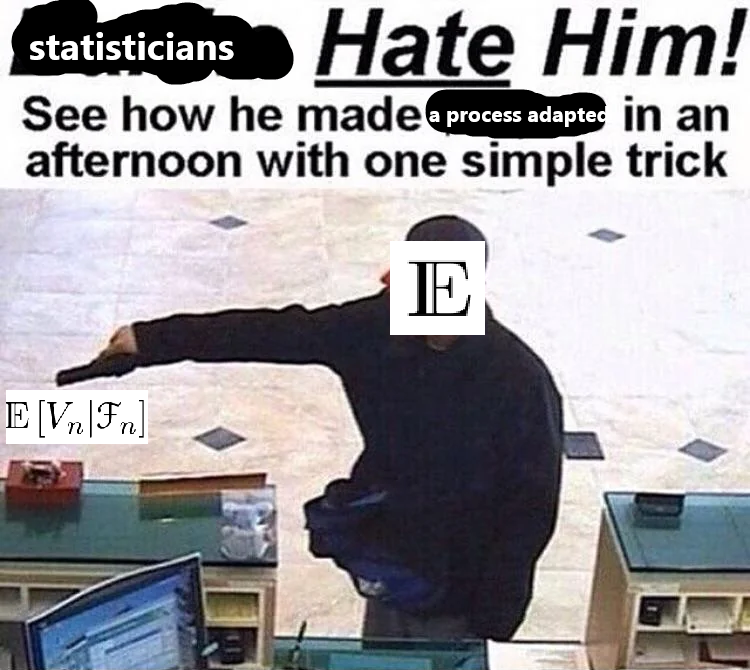
\includegraphics[width=0.7\linewidth]{screenshot009}
		\caption{You conditioned in the wrong hood, buddy.}
		\label{fig:screenshot009}
	\end{figure}
	\subsection{Stopping times}
	Consider now the same problem under a different point of view: we want to establish the ``best time'' when to stop discarding candidates. This is a random time and it is called a \emph{stopping time}. This is nothing else than a time that we choose basing ourselves on elements or events that may or may not happen: this is why they're a \rv. The stopping times are a random variable that can cause problems, since stopping times can be infinite: imagine that our stopping time is "whenever a volcano erupts" but the stupid fucking volcano decides to go into quiescence forever. This is why beside our index set $\T$ we need to introduce $\Tbar=\T\cup\{\infty\}$.
	\begin{definition}
		\[T:\Omega\mapsto\Tbar
		\]
		is called \emph{stopping time} of $\F$ if
		\[\{T\leq t\}\in\F_t\qquad\every t\in\T.\]
	\end{definition}
	Remember that stopping times have to be $\F$-measurable: for example "when will the fucking volcano erupt for the last time" is \textit{not} a stopping time because it requires information that we don't have in $t$! \\
	Stopping time have an alternative definition:
	\begin{definition}
		$T$ is a stopping time if the process
		\[Z_t=\indi_{\{T\leq t\}}\qquad t\in\T\]
		is adapted to $F$.
	\end{definition}
	From this definition it follows that when $\T=\N$ then this is equivalent to having
	\[\underbracket[0.6pt]{\hat{Z}_{n}}_{\mathclap{Z_n-Z_{n-1}}}=\indi_{\{T=1\}}\qquad\every n\in\N\]
	that needs being adapted to $\F_n$.\\
	Not all random times are stopping time: think about an experiment in which we produce a signal when a physical event happens. Let us call $Z$ the process indicator and $T$ our stopping time:
	\[Z_t{\omega}=\begin{cases}
		0&t<T(\omega)\\
		1&t\geq T(\omega).
	\end{cases}\]
	Then if the information flow allows us to recognize the occurrence of the event then $T$ is a stopping time.
	\begin{example}
		Some stopping times:
		\begin{enumerate}[\circnum]
			\item The first time that $X(\omega)\in H\in\Omega$;
			\[T(\omega)=\begin{cases}
				\inf \left\{n\in\N:X_n(\omega)\in H\right\}&\\
				+\infty&\text{if $X_n(\omega)\notin H\;\every n$}
			\end{cases}\]
			So
			\[\left\{T\leq n\right\}=\bigcup_{k=0}^{n}\left\{X_k\in H\right\}.\]
			\item Consider i.i.d. \rv{}s 
			$X_1,X_2,\ldots$. Consider the probabilities
			\[\pr(X_i=1)=\pr(X_i=-1)=\frac{1}{2}\]
			and the random walk
			\[S_n=\sum_{1}^{n}X_i.\]
			Let's define 
			\[T_1=\begin{cases}
				\min\left\{n<50:S_n=3\right\}\\
				50 &\text{otherwise}.
			\end{cases}\]
			This is a stopping time because I can write $\left\{T_1\leq n\right\}$ as $$\underbracket[0.6pt]{\bigcup_{k=1}^{n}\underbracket[0.6pt]{\left\{S_k=3\right\}}_{\text{$\F_k$-measurable}}}_{\mathclap{\text{$\F_n$-measurbale}}}\qquad n<50.$$
			Moreover for $n=50$ we have $T_{1}\in\F_{50}$.
			\item Starting from the previously deifned random walk, consider the quantity 
			\[M_n=\min(S_1,\ldots,S_n)\]
			And the random time
			\[T_2=\min\left\{n:S_n\geq M_m+2\right\}\]
			is a stoppimg time. On the contrary, 
			\[T_3=\begin{cases}
				\max\left\{n<50:S_n=7\right\}&\text{if not empty}\\
				50 &\text{otherwise}
			\end{cases}\]
			is not a stopping time. Why? Because I have to wait until $n=50$ to answer the question. 
		\end{enumerate}
	\end{example}
	
	Consider the random times on $\R_+$
	\[0<T_1<T_2<\ldots\]
	With $\lim_{n\to\infty}T_n=+\infty$. Define the process $\left\{N_t\right\}$ as 
	\[N_t:=\sum\indi_{[0,t]}(T_n).\]
	This is called \emph{counting process}. It is a basic count of the number of events happened up to time $n$.
	\begin{figure}[H]
		\centering
		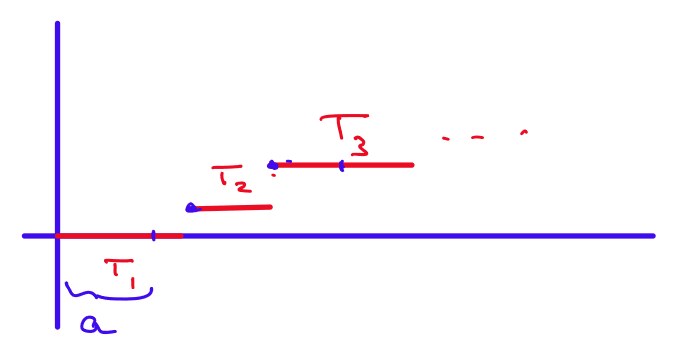
\includegraphics[width=0.6\linewidth]{screenshot010}
		\caption{Yeah I'm counting on ending my life very soon.}
		\label{fig:screenshot010}
	\end{figure}
	$N_{t}$ is increasing, right continuous and incresases by unitary jumps. Moreover, $N_0=0$, $N_t<\infty$ for $t\in\R_+$. Of course $\lim_{t\to\infty}N_t=\infty$. Counting processes generate their natural filtration $\F$.
	
	Some problems require to stop the observation at a stopping time (because we don't care anymore\footnote{Assuming we ever did.})... So we don't actually need the whole knowledge of the complete filtration $\F={\left(\F_t\right)}_{t\geq 0}$. The problem is that as we said before the stopping time is a random time. So what we need is the \textit{information known up to time $T$} $\F_T$, basically the $\sigma$-field that is the filtration at time $T$. 
	\begin{remark}
		We said that $\F_t$ does not include $t=\infty$... but $T$ may diverge to $\infty$! We need to enlarge $\F$ to include $t=\infty$.
	\end{remark}
	Think, for instance the stopping time ``first time of overflowing of a dam''. It is something that may very well never happen and is therefore called ``Vajont stopping time\footnote{Okay I'm sorry I'm sorry I am a terrible person yes sir yes yes I concur it was an extremely inappropriate joke yes yes sir yes you have my word yes no no never again no you don't have to worry no no.}''.
	\begin{definition}
		Let $\Tbar=\T\cup\left\{+\infty\right\}$. We define
		\[\F_\infty=\lim_{t\to\infty}\F_t=\underbracket{\bigvee_{t\in\T}\F_+}_{\sigma\left(\bigcup\F_t\right)}.\]
	\end{definition}
	\begin{definition}
		$\F_{\Tbar}$ is a filtration on $\Tbar$ and $T$ is a stopping time on it if and only if it is a stopping time on $\F_\T$.
	\end{definition}
	\begin{remark}
		Every stochastic process on ${(\F_{t})}_{t\in\T}$ can be extended to $\Tbar$ by appending any \rv{} $X_\infty$ to it (with $X_\infty\in\F_{\infty}$).
	\end{remark}
	So adding this \rv{} doesn't really add any information but only ensures that nerds don't whine about completeness. It is \textit{technically} information that we will never user, since $\F_\infty$ does not contain any further information with respect to $\F$. We denote with $\F$ also the extended filtration, with the ease of mind given by the fact that a divergent stopping time won't make us commit harakiri.
	\begin{definition}
		Let $\F$ be a filtration on $\Tbar$ and let $T$ be a stopping time on $\F$. We call \emph{past until $T$} the \sa{} $\F_t\subset\F_\infty\subset\HS$ such that:
		\[\F_T=\left\{H\in\HS:H\cap\{T<t\}\in\F_t,\every t\in\Tbar\right\}.\]
	\end{definition}
	This means that $\F_T$, which represents the evolution within $T$, contains all the events $H$ such that they are before the stopping time in all the filtrations. This is selecting the events $H$ that happen within the time $T$.
	\begin{remark}
		If we fix a $T\equiv t$ then $\F_T\equiv\F_t$ (it's the normal filtration at time $t$).
	\end{remark}
	If $T$ is a stopping time of $\F$ then $\{T\leq r\}$ belongs to $\F_T,\;\every r\geq 0$:
	\[\{T\leq r\}\cap\{T\leq t\}=\{T\leq\min(T,r)\}\in\F_t\]
	So $T$ is $\F_T$-measurable. 
	\begin{remark}
		$\F_t$ can be read as the collection of all $\F_t$-measurable \rv{}s $V$: the value of $V(\omega)$ can be told by the time $T(\omega)$: we can read the value of $V(\omega)$ before the ringing of an alarm.
	\end{remark}
	\begin{theorem}
		A random variable $V$ belongs to $\F_T$ if and only if
		\begin{equation}
			V\indi_{T\leq t}\in\F_t,\qquad\every t\in\Tbar.\tag{$i$}\label{stopstopstop}
		\end{equation}
		If $\Tbar\equiv\overline{\N}$ the condition becomes
		\begin{equation*}
			V\indi_{T=n}\in\F_n\qquad\every n\in\overline{\N}.
		\end{equation*}
	\end{theorem}
	\begin{fancyproof}
		Note that 
		\[X_t=V\indi_{T\leq t}\]
		is a stochastic process. For $\every r\in\R_+$ and $t\in\T$
		\[\{V>r\}\cap\{T\leq t\}=\{X_t>r\}.\]
		But now we know that (\ref{stopstopstop}) is just a consequence of the definition of $\F_t$:
		\[\{V>r\}\in\F_T\quad\every r\underset{\text{def. of $\F_T$}}{\iff}\{X_t>r\}\in\F_t\qquad\every r,\every t\in\Tbar\]
		The special case in which $\Tbar\equiv\overline{\N}$ means that
		\[V\indi_{\{T=n\}}=\begin{cases}
			X_n-X_{n-1}&\text{if }n\in\N\\
			X_\infty-\sum_{n\in\N}(X_n-X_{n-1})&\text{if }n=\infty
		\end{cases}\]
		so that 
		\begin{equation*}
			V\in\F_T\iff V\indi_{T=n}\in\F_n
		\end{equation*}
	\end{fancyproof}
	But what if there is a problem that involves more than 1 stopping time? We cannot use two different ``pasts'' because that would cause problems with the measurability of \rv s. 
	\begin{example}
		Imagine a factory. The production is blocked when
		\begin{enumerate}[a)]
			\item the temperature of the room is above a certain threshold; 
			\item the machinery has not been cleaned for more than 12 hours.
		\end{enumerate}\par
		Alternatively, imagine that the sales of shares happens:
		\begin{enumerate}[a)]
			\item when the price is above a fixed value;
			\item when the increase of the price is smaller than a fixed value.
		\end{enumerate}
	\end{example}
	Both of this cases require the use of 2 different stopping times $S$ and $T$. We may think to evaluate two typical functions of $S$ and $T$ of interest:
	\begin{equation*}
		\underbrace{\min\{S,T\}}_{S\wedge T}\qquad	\underbrace{\max\{S,T\}}_{S\vee T}
	\end{equation*}
	\begin{example}
		\emph{Truncated stopping time}: let $T$ be a stopping time (for example, the time at which we sell certain shares) and that we want a finite horizon for this decision. In this case the quantity of interest is
		\begin{equation*}
			S=T\wedge n=\min\{T,n\}
		\end{equation*}
		where $n$ could be some sort of time horizon.\\
		Imagine that two cyclists participate to a race. Their children will have their snack when both the parents will arrive to the finish line. How long will the children wait for their snack?
		We can think about the following stopping times:
		\[ 	\begin{array}{l l}
			T: & \text{time employed by the first cyclist}\\
			S: & \text{time employed by the second cyclist}\\
			U: &\max\{S,T\}.
			
		\end{array} \]
		The waiting time for the children will be $U$.
	\end{example}
	This is cool and all, but are we sure that $S\wedge T$ and $S\vee T$ are stopping times?
	\begin{remark}
		Yes.
	\end{remark}
	Why?
	\begin{remark}
		Fuck you.
	\end{remark}
	Aw hell nah. Now even the color boxes are against me. 
	\begin{insult}
		You will NEVER pass this exam.
	\end{insult}
	Well this is not a surprise.
	\begin{insult}
		Not if you keep jerking around.
	\end{insult}
	\begin{fancyproof}
		We know that $\{S\leq t\}$ and $\{T\leq t\}$ belong to $\F_t$ for every $t$, since they are stopping times. Consider now $\left\{\min\{(S,T)\leq t\}\right\}$ and $\left\{\max\{(S,T)\leq t\}\right\}$. We have
		\begin{equation*}
			\left\{\min\{(S,T)\leq t\}\right\}=\underbrace{\underbrace{\{S\leq t\}}_{\in\F_t}\cup\underbrace{\{T\leq t\}}_{\in\F_t}}_{\in\F_t}
		\end{equation*}
		and 
		\begin{equation*}
			\left\{\max\{(S,T)\leq t\}\right\}=\underbrace{\underbrace{\{S\leq t\}}_{\in\F_t}\cap\underbrace{\{T\leq t\}}_{\in\F_t}}_{\in\F_t}.
		\end{equation*}
	\end{fancyproof}
	There is a further theorem:
	\begin{theorem}
		\begin{enumerate}[\circnum]
			\item if $S\leq T\implies\F_S\subset\F_T$;
			\item $\F_{\min\{S,T\}}=\F_S\cap\F_T$;
			\item if $V\in\F$, the following processes are in $\F_{\min\{S,T\}}$:
			\begin{equation*}
				\begin{array}{c c c}
					\color{SteelBlue4}(a)&\color{SteelBlue4}(b)&\color{SteelBlue4}(c)\\
					V\indi_{S\leq T},&V\indi_{S=T},&V\indi_{S< T}.
				\end{array}
			\end{equation*}
		\end{enumerate}
	\end{theorem}
	\begin{fancyproof}
		\begin{enumerate}
			\item Imagine $\{S\leq T\}$. Now consider the event $\{S\leq n\}$. Since $S$ happens before $T$ then we have that $\{T\leq n\}\subset\{S\leq n\}$. We know that if $A\in\F_S$ then
			\[A\cap\{T\leq n\}=A\cap\underbracket[0.6pt]{\{S\leq n\}}_{\in\F_n}\cap\underbracket[0.6pt]{\{T\leq n\}}_{\in\F_n}\]
			which means that $A\cap\{T\leq n\}\in\F_n$ and by definition of $\F_T$
			this correponds to saying
			\[\F_S\subset\F_T.\]
			\item \begin{enumerate}
				\item Let us first prove that $\F_{\min\{S,T\}}\subset\F_{S}\cup\F_T$.
				Note that $\min\{S,T\}$ is dominated by $\F_s$ and $\F_T$, which means that $\F_{\min\{S,T\}}$ is included both in $\F_S$ and $\F_T$. By point 1 we have
				\[\F_{\min\{S,T\}}\subset\F_S\cap\F_T.\]
				\item It remains to prove that $\F_{\min\{S,T\}}\supset\F_{S}\cup\F_T$. Let $H\in\F_S\cap\F_T$. This means that 
				\begin{equation*}
					H\cap\{S\leq T\}\in\F_{\min\{S,T\}}
				\end{equation*}
				by part the of this theorem, since $H\in\F_S$. But we also know that
				\[H\cap\{T\leq S\}\in\F_{\min\{S,T\}}\]
				by part 3 of this theorem since also $H\in\F$. But this means that
				\begin{equation*}
					H=\left\{H\cap\left\{S\leq T\right\}\right\}\cup\left\{H\cap\left\{S\leq T\right\}\right\}
				\end{equation*}
				belongs to $\F_{\min\{S,T\}}$ and so
				\[\F_{\{S\cap T\}}\subset\F_{\min\{S,T\}}.\]
			\end{enumerate}
			\item\begin{enumerate}
				\item $V\indi_{\{S\leq T\}}\in\F_{\min\{S,T\}}$. To prove this we use the following theorem:
				\begin{theorem}
					Let $T$ be a stopping time of $\F$. Then
					\[\F_T=\{X_T:X\in\F\}\]
					with $X$ in $\F$.
				\end{theorem}
				This baiscally means that $\F_t$ becomes the values $X_T$ of $X$ in $\F$ at time $T$. Let us consider $X_t=V\indi_{\{S\leq t\}}$ with $t=\min\{S,T\}$. We know that $\min\{S,T\}$ is a stopping time of $\F_{\min\{S,T\}}$ and by the theorem above
				\[X_{\min\{S.T\}}\in\F_{\min\{S,T\}}\]
				or, alternatively,
				\[\indi_{\{S\leq T\}}\in\F_{\min\{S,T\}}.\]
				\item Let $V=2\implies\{S\leq T\}\in\F_{\min\{S,T\}}$ and by symmetry $\{T\leq S\}\in\F_{\min\{S,T\}}$. This means that 
				\begin{equation*}
					\{S=T\}=\{S\leq T\}\cap\{T\leq S\}\in\F_{\min\{S,T\}}.
				\end{equation*}
				Furthermore 
				\[\{S<T\}=\{S\leq T\}\setminus\{S=T\}\]
				Which implies memebership of $\F_{\min\{S,T\}}$.
				\item Consider the fact already proven that $V\indi_{\{S\leq T\}}\in\F_{\min\{S,T\}}$. Multiplying by $\indi_{\{S=T\}}$ or $\indi_{\{S<T\}}$ does not alter the membership in $\F_{\min\{S,T\}}$.
			\end{enumerate}
		\end{enumerate}
	\end{fancyproof}
	Consider now a machinery what when it becomes too hot (above a certain threshold) an alarm rings and after 3 seconds the machinery stops. Here we deal with 2 times:
	\begin{equation*}
		\begin{array}{l l}
			T: &\text{time of the alarm (stopping time)}\\
			t=3: &\text{deterministic time (stopping time as well)}\\
		\end{array} 
	\end{equation*}
	and the time of our interest is the time $S$ when the machinery stops:
	$$S=T+t$$
	\begin{remark}
		At time $T$ we know $S$: We know that when the alarm rings within three seconds the machinery will stop, so $S$ is actually $\F_T$-measurable. We say that \emph{$S$ is foretold by $T$}.
	\end{remark}
	\begin{definition}
		Let 
		\begin{equation*}
			\begin{array}{l l}
				S &\text{be a stopping time}\\
				T &\text{be a random time $T>S$ but whose value can be told by time $S$.}
			\end{array}
		\end{equation*}
		We say that $T$ is \emph{foretold by $S$} (and it is a stopping time).
	\end{definition}
	\begin{example}
		Consider $S$ and $T=2S$. Surprise surprise, $T$ is a foretold time.
	\end{example}
	Did we need an example for this?
	\begin{example}
		Yes.
	\end{example}
	Yeah this meta-joke has been running long enough.
	\subsection{Discrete and continuous stopping times}
	\begin{definition}
		Let
		\begin{equation*}
			d_n(t)=\begin{cases}
				\frac{k+1}{2^{n}}&\text{if }\frac{k}{2^{n}}\leq t <\frac{k+1}{2^{n}}\\
				+\infty &\text{if }t=\infty.
			\end{cases}
		\end{equation*}
		We got a function
		\[d_n:\Rext_+\mapsto\Rext_+.\]
	\end{definition}
	Consider the case $n=1$ (remember that $k=0,1,2,\ldots$):
	\begin{figure}[H]
		\centering
		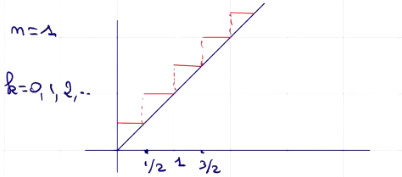
\includegraphics[width=0.6\linewidth]{screenshot011}
		\caption{These are screenshots taken from the video feed. I couldn't bother. Sorry.}
		\label{fig:screenshot011}
	\end{figure}
	But after $n=2$ we get the same function with smaller "steps":
	\begin{figure}[H]
		\centering
		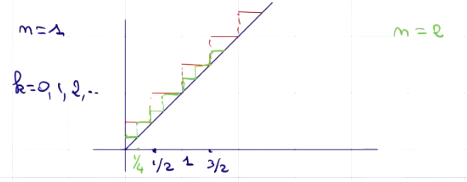
\includegraphics[width=0.6\linewidth]{screenshot012}
		\caption[The problem of improvisation]{The aesthetic problem of musical execution is reduced by Enrico Fubini to a problem of musical improvisation: I honestly think that this perspective is limiting both in its conceptions of ``execution'' and ``improvisation'' even if I agree with the intent of blurring the line between the two concepts unjustly separated in our Western modern musical. That is, a modern perspective: the reader will surely remember that Bach was famous first and foremost for his improvisational abilities and that the musical form of the fugue was often used to display pyrotechnical capabilities in that regard.}
		\label{fig:screenshot012}
	\end{figure}
	Observe that $d_1\geq d_2\geq d_3\geq\ldots$. What are the other properties of this function?
	\begin{enumerate}
		\item it is a step function;
		\item it is right-continuous;
		\item $d_n(t)>t$ (the diagonal line);
		\item $\lim_{n\to\infty}d_n(t)=t$.
	\end{enumerate}
	Now we apply this simple function to our stopping times so that we get the following proposition.
	\begin{proposition}
		Let $\F$ be a filtration on $\Rext_+$ and let $T$ be a stopping time. Let 
		\[T_n=d_n\circ T.\]
		Then ${\{T_n\}}_{n}$ is a sequence of \emph{discrete stopping times} of $\F$ decreasing to $T$.
	\end{proposition}
	\begin{remark}
		Of course $T_n$ is a foretold time by $T$, because if I know $T$ I also know the value of $T_n$.
	\end{remark}
	\begin{fancyproof}
		Fix $n$:
		\begin{itemize}
			\item $T_n$ is a measurable function of $T\implies T_n\in\F_n$;
			\item $d_n(t)\geq t\quad\every t<\infty$ and $d_n(\infty)=\infty\implies d_n(T)=T_n\geq T$;
			\item $T_n$ is a foretold time by $T$;
			\item $T_n$ is a stopping time;
			\item $T_n$ is discrete.
		\end{itemize}
		But $d_n(t)\searrow t$ as $n\to\infty\implies d_n(T)=T_n\searrow T$. We have thus switched from a continuous stopping time to a sequence of discrete stopping times.
	\end{fancyproof}
	An important thing to note is that during our process of discretization we never break the property of the stopping times... and this is possible because we are using foretold times!
	\subsection{Conditioning at stopping times}
	Imagine that we have our information about $X$ that stops at the stopping time $T$: this means knowing $\F_T$. Consider the classic conditioning situation
	\[\ev(X\F_T).\]
	We already said how this is our best estimate of $X$ using our information available (that is $\F_T$).
	\begin{notation}
		We will write
		\[\ev_T\equiv\ev_{\F_T}\equiv\ev(\cdot|\F_T).\]
	\end{notation}
	\begin{remark}
		Can I use $T$ fixed as a deterministic time $t$ and thus get $\ev(X|\F_t)$? Is this a special case or a different think altogether? Well yes, because $t$ \textit{is} a stopping time being $\F_t$-measurable! $\ev(X|\F_t)$ is a special case of $\ev(X|\F_T)$.
	\end{remark}
	This becomes clear when we see the properties of stopped expectation. For $\every X,Y,Z$ being positive \rv s and for $\every S,T$ stopping times of $\F$ the following properties hold:
	\begin{itemize}
		\item \emph{defining property}:
		\[\ev_T X=Y\iff V\in\F_T\text{ and }\ev VX=\ev VY;\]
		\item \emph{unconditioning}:
		\[\ev\ev_T X=\ev X;\]
		\item \emph{repeated conditioning}:
		\[\ev_S\ev_T X=\ev_{\min\{S,T\}}X=\ev_{S\wedge T}X;\]
		\item \emph{conditional determinism}:
		\[\ev_T(X+YZ)=X+Y\ev_T(Z)\]
		if $X,Y\in\F_T$.
	\end{itemize}
	We need to prove the third property.
	\begin{fancyproof}
		Notice that if $S\leq T\implies\F_S\subset\F_T$. This means that 
		\[\ev_S\ev_T=\ev_S\left(=\ev_{S\wedge T}\right)\]
		(the ``poorer'' \sa{} wins!). Moreover notice that if $S$ and $T$ are arbitrary we can apply the same result to $S\wedge T$ since $S\wedge T\leq T$ and 
		\begin{equation}
			\ev_{S\wedge T}\ev_{T}=\ev_{S\wedge T}\tag{$\bullet$}\label{stopexpect}
		\end{equation}
		Remember that $Y=\ev_T X$. Let's now try to write the statement of our proof in a different way:
		\[\ev_S Y=\ev_{S\wedge T}X.\]
		But using our property (\ref{stopexpect}) we get
		\begin{align*}
			\ev_S Y&=\ev_{S\wedge T}\ev_T X\\
			&=\ev_{S\wedge T} Y.
		\end{align*}
		Let's prove this, by steps.
		\begin{enumerate}
			\item note that $\F_{S\wedge T}\subset\F_S$. This means that $\ev_{S\wedge T}Y$ is in $\F_S$ and therefore $\ev_{S\wedge T}Y $ has the measure property and it is a candidate to be $\ev_S Y$. So we should check whether this candidate satisfies the defining property of stopped expectation.
			\item Check the defining property
			\[\ev VY=\ev V\ev_{S\wedge T}Y\]
			for each positive $V$ in $\F_S$. We start by fixing such $V$, positive and in $\F_S$. We proved that 
			\[V\indi_{\{S\leq T\}}\in\F_{S\wedge T}\]
			and the defining property for $\ev_{S\wedge T}$ gives
			\begin{equation}
				\ev V\indi_{\{S\leq T\}}Y=\ev V\indi_{\{S\leq T\}}\ev_{S\wedge T}Y\tag{$\bullet\bullet$}\label{hateproof}
			\end{equation}
			Now we observe that $Y\in\F_T$ by definition. Also notice that $Y\indi_{\{T<S\}}\in\F_{S\wedge T}$. Apply now this fact to the defining property and obtain
			\begin{equation*}
				\ev VY\indi_{\{T<S\}}=\ev V\ev_{S\wedge T}Y\underbracket{\indi_{\{T<s\}}}_{\mathclap{\F_{S\wedge T}\text{-meas.}}}
			\end{equation*}
			and by conditional determinism we get
			\begin{align*}
				\ev VY\indi_{\{T<S\}}&=\ev V\indi_{\{T<S\}}\\
				&=\ev V\indi_{\{T<S\}}\ev_{S\wedge T}Y.
			\end{align*}
			By putting together this result with (\ref{hateproof}) we get
			\begin{equation*}
				\ev V Y=\ev V\ev_{S\wedge T}Y.
			\end{equation*}
		\end{enumerate}
	\end{fancyproof}
	\section{Martingales}
	When we study stochastic processes, the typical way of introducing classes of stochastic processes for which we have methods to study is determining the finite dimensional distributions. If we have them, thanks to the Kolmogorov Consistency theorem, we can give a complete description of the process but this is boring and for fucking losers. So we introduce classes of stochastic processes for which we can write the distribution.\par
	Imagine, from a different view point, another approach: instead of starting from the distribution of a stochastic process we start from a property; then as a consequence of that property we infer the behavior towards infinity. This is the philosophy behind the class of \emph{martingales}.
	\begin{example}
		Consider the process $\{X_{n}\}$ that describes the fortune of a player. This player wins with probability $p$ and loses with probability $1-p=q$. Consider the fortune at time $n$ ${\{S_n\}}_{n\geq 0}$, which is 
		\[S_n=\sum_{i=0}^{n}X_i.\]
	\end{example}
	Is the game fair? Imagine also that the $X_i$'s are the value that I get by losing or selling options or stock. We know that the game is fair if $p=q=\frac{1}{2}$. But this could also be written as a property in the following way:
	\[\ev\left[S_{n+1}|\underbracket[0.64pt]{S_n}_{\F_n}\right]=S_n.\]
	So I don't have any ``advantages'' or ``bias''.
	\begin{fancyproof}
		\begin{align*}
			\ev\left[S_{n+1}|S_n\right]&=\ev\left[S_n+X_{n+1}|S_n\right]\\
			&=S_n+\ev\left[X_{n+1}|S_n\right]\\
			&=S_n+\underbracket[0,6pt]{\ev\left[X_{n+1}\right]}_{\mathclap{=0\text{ if }p=q=\frac{1}{2}}}\\
			&=S_n
		\end{align*}
	\end{fancyproof}
	We will not define martingales through the event/filtration that allows the process $Y$ to remain constant:
	\[\ev[Y_{n+1}|\F_n]=Y_n.\]
	Then we should ask some questions about this \sa. We know that $\{\F_n\}$ can be increasing, constant or decreasing but $Y$ must remain constant in mean. Look at it through the tower property.
	\[\ev Y_n=\ev\left[\ev\left[Y_{n+1}|\F_n\right]\right]=\ev Y_{n+1}.\]
	\begin{definition}
		A real-valued process
		\[X={(X_t)}_{t\in\T}\]
		is called a \emph{$\F$-martingale} if:
		\begin{enumerate}
			\item it is adapted to $\F$;
			\item it is integrable for each $t\in\T$;
			\item $\ev(X_t-X_s|\F_s)=0\quad\every s<t$.
		\end{enumerate}
		If $\ev(X_t-X_s|\F_s)\geq0\quad\every s<t$ then the process is called \emph{$\F$-submartingale} and if $\ev(X_t-X_s|\F_s)\leq0\quad\every s<t$ it is called \emph{$\F$-supermaringlae}.
	\end{definition}
	These three properties are what we need to check to establish whether a process has martingale properties. The first two are really just regularity conditions, while the third is the ``real'' defining property of a martingale. There is is another definition for the third property:
	\begin{definition}
		\begin{enumerate}
			\item[3'.] $\ev(X_t|\F_s)=X_s$.
		\end{enumerate}
	\end{definition}
	In the first definition we were looking at the increment, now we are looking at the mean of a further point $t$ in time for the process $X$ and discovering that, conditioning it to information available in time $s$, it doesn't change from the process in time $s$.\\
	If $\ev X^{+}_{t}<\infty$ then the sequence $\{X_t\}$ (that can be a sub-martingale) converges to a limit. 
	\begin{remark}
		A martingale is also a sub-martingale and a super-martingale.
	\end{remark}
	We will use sub-martingales in our demonstrations but it really does not change anything because if $\{X_t\}$ is a $\F$-sub-martingale then $\{-X_t\}$ is a $\F$-super-martingale.
	\begin{remark}
		The number of terms in $\{X_t\}$ can be bounded or unbounded: even a process with 4 terms can be a martingale.
	\end{remark}
	There are consequence to the way we defined martingales. Consider the times $s<t<u$ and the $\F$-martingale $\{X_t\}$. Then
	\[\ev_s(X_u-X_{t})\]
	means knowing the evolution of the process at time $s$ and looking for the increment of the process between $t$ and $u$. 
	\begin{figure}[H]
		\centering
		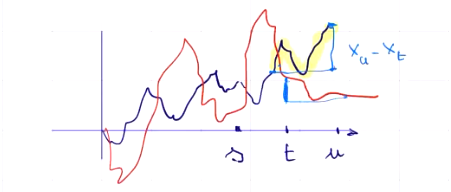
\includegraphics[width=0.7\linewidth]{screenshot013}
		\caption{It should not}
		\label{fig:screenshot013}
	\end{figure}
	We can write
	\begin{align*}
		\ev_s(X_u-X_{t})&=\ev_s\Big(\underbracket[0.56pt]{\ev_t(X_u-X_t)}_{\mathclap{=0\text{ bc it is a martingale}}}\Big)\\
		&=\ev_s 0=0.
	\end{align*}
	This means that given the information up to time $s$ the estimation of any future increment will be null! In the special case $\T=\N$ then this property becomes
	\[\ev_n(X_{n+1}-X_n)=0.\]
	\begin{proposition}
		If $\{X_i\}$ is an $\F_n$-martingale, it holds
		\[\begin{array}{l l}
			\ev X_i=\ev X_{i+1}&\text{if it is a martingale}\\
			\ev X_{i+1}>\ev X_i&\text{if it is a sub-martingale.}
		\end{array}\]
	\end{proposition}
	\begin{fancyproof}
		Consider the expectation
		\[\ev(X_{i+1}|\F_i)\geq X_i\]
		being a sub-martingale. Take the expectation
		\[\underbrace{\ev\left[\ev(X_{i+1}|\F_i)\right]}_{\ev X_{i+1}}\geq\ev X_i.\]
		We can now define the process
		$\{Y_{i}\}_{i\in\N}$ as 
		\[Y_{i+1}=X_{i+1}-X_{i}.\]
		We know that $\{X_i\}$ is a $\F$-martingale. Note that
		\[\sum_{j=1}^{i} Y_j=X_1-X_0+X_2-X_1+\ldots+X_i-X_{i-1}\]
		so that we can write
		\[X_i=c+\sum_{j=1}^{i}Y_j.\]
		We know that 
		\[\ev\left[X_{i+1}|\F\right]=X_i\]
		But we also know that 
		\begin{equation*}
			\ev[Y_{i+1}|\F]=0.
		\end{equation*}
	\end{fancyproof}
	The quantity $\{\ev{Y_{i+1}|\F_i}\}$ is called \emph{martingale difference}.
	\begin{example}
		Imagine we have a sequence $\{Y_i\}$ of independent \rv s with $\ev Y_i=0$.
		Consider $\F_1$, the \sa{} generated by $\{Y_j,0\leq j\leq i\}$. Call $S_i=c+\sum^{i}Y_{j}$. 
		$\{S_i\}$ is an $\F$-martingale.
	\end{example}
	\subsection{Properties of martingales}
	\begin{enumerate}
		\item Consider $X$ and $Y$ being $\F$-sub-martingales and $a,b\in\R^{+}$. Then 
		\[aX+bY\]
		is a $\F$-sub-martingale.
		\item Consider $X,Y$ being two $\F$-sub-martingales. Then
		\[\max\{X,Y\}\]
		is a $\F$-sub-martingale.
		\begin{fancyproof}
			Consider $\ev[\max\{X_{n},Y_{n}|\F_{n-1}\}]$. Remember that we have to prove: \begin{itemize}
				\item measurability property;
				\item integrability property;
				\item martingale property.
			\end{itemize}
			Often times measurability and integrability are implied in the form of the function.  Since we are using the maximum between $X$ and $Y$ we know that
			\[\begin{array}{l}
				\ev[\max\{X_{n},Y_{n}|\F_{n-1}\}]\geq\ev[X_{n}|\F_{n-1}\}]\\
				\ev[\max\{X_{n},Y_{n}|\F_{n-1}\}]\geq\ev[Y_{n}|\F_{n-1}\}].
			\end{array}\]
			But since $X$ and $Y$ are martingales we know that $\ev[X_{n}|\F_{n-1}]\geq X_{n-1}$ and $\ev[Y_{n}|\F_{n-1}]\geq Y_{n-1}$; hence we get that
			\[\ev[\max\{X_{n},Y_{n}|\F_{n-1}\}]\geq\max\{X_{n-1},Y_{n-1}\}\]
			so the martingale property is satisfied.
		\end{fancyproof}
		\item Consider two $\F$-super-martingales $X_{n},Y_{n}$. Then
		\[\min\{X_{n},Y_{n}\}\]
		is a $\F$-super-martingale.
		\begin{fancyproof}
			Consider $\max\{-X_{n},-Y_{n}\}$. We know that $-X_n$ is a sub-martingale and so is $-Y_{n}$. So as proved above $\max\{-X_{n},Y_{n}\}$ is a sub-martingale. But $\max\{-X_{n},-Y_{n}\}=-\min\{X_{n},Y_{n}\}$ so
			\[-\min\{X_{n},Y_{n}\}\text{ is a sub-martingale}\iff\min\{X_{n},Y_{n}\}\text{ is a super-martingale}.\]
		\end{fancyproof}
		\item Consider a function $f$ that is \underline{convex} on $\R$. If $X$ is a $\F$-martingale and $f\circ X$ is integrable then $f\circ X$ is a $\F$-sub-martingale.
		\begin{fancyproof}
			We have $s<t$ and we want to study $\ev\left[f(X_{t})|\F_{s}\right]$. By Jensens's inequality we have
			\begin{align*}
				\ev\left[f(X_{t})|\F_{s}\right]&\geq f\Big[\underbrace{\ev(X_{t}|\F_s)}_{X_s}\Big]\\
				&=f(X_s).
			\end{align*}
		\end{fancyproof}
		\begin{remark}
			Some examples of positive functions of $X$ are $X^{+},X^{-},|X|$. If $X$ is martingale, these are sub-martingales.  $|X|^{p}$ is a sub-martingale if $X$ is a martingale and $\ev|X|^{p}<\infty$.
		\end{remark}
		\item if $f$ is convex and increasing and $X$ is a $\F$-sub-martingale with $f(X_{t})$ integrable $\every t$ then $f(X_{t})$ is again a $\F$-sub-martingale.
	\end{enumerate}
	\subsection{Create your own martingale}
	\begin{enumerate}
		\item Consider an increasing family of \sa s $\{\F_j\}$ and a \rv{} $X$ on $(\Omega,\F,\pr)$ which is integrable and adapted to $\F$.
		Define 
		\[X_i=\ev[X|\F_i].\]
		Then the process ${\{X_i\}}_{i\in\N}$ is called \emph{Doob martingale} and plays an important role in may processes. As $i$ increases, so does the information about our random variable while retaining the underlying process $X$.\\
		We have now to prove that $\{X_i\}$ is a $\F$-martingale. 
		\begin{fancyproof}
			We need to check that \begin{align*}
				\ev[X_{i+1}|\F_{i}]&=\ev\left[\ev\left[X|\F_{i+1}\right]|\F_{i}\right]\\
				&=\ev\left[X|\F_{i}\right]
			\end{align*}
			and this is because of the properties of conditional expectation since $\F_{i+1}\supset\F_{i}$. But $\ev\left[X|\F_{i}\right]=X_i$ by definition.
		\end{fancyproof}
		The same result holds when $\T$ is continuous.
		\item Consider sums of independent \rv $\{X_i\}$ with $\ev[X_i]=0$. We have 
		\[S_0=0\qquad S_n=S_0+X_1+X_2+\ldots+X_{n}\qquad n\geq1.\]
		We define $\F={(\F_{n})}_{n\in\N}$ as the filtration generated by $S={(S_{n})}_{n\in\N}$. Consider the following facts:
		\begin{enumerate}
			\item $\F_{n}$ is adapted to $S$;
			\item Each $S_{n}$ is integrable and $\ev S_{n}=0$;
			\item $\ev_{n}(S_{n+1}-S_n)=\ev_n(X_{n+1})=\ev X_{n+1}=0$ (because of independence).
		\end{enumerate}
		So $S_{n}$ is a martingale.
		What happens, tough, if $\ev X_i=1$ for each $i$? We would get a sub-martingale (because we would have an increasing process).
		\item Consider the product of \rv s. Consider $R_1,R_2,\ldots$ being independent \rv s with
		\[\ev R_i=1\qquad\var R_i<\infty\]
		that don't necessarily need to be identically distributed. Let $M_{0}=1$ and $M_n=M_{0}\cdot R_{1}\cdot R_{2}\cdot\ldots\cdot R_{n}$ and let $\F$ be the filtration generated by $M={\{M_n\}}_{n\in\N}$. Observe that
		\begin{enumerate}
			\item $M$ is adapted to $\F$ by definition;
			\item $\every M_{n}$ is integrable: consider $\norm{M_{n}}\leq\norm{M_{n-1}}\norm{R_{n}}$ since $M_{n}=M_{n-1}R_{n}$. But since $R_{n}$ has finite variance then $\norm{M_{n-1}}\norm{R_{n}}<\infty$. So since it is bounded it is integrable;
			\item consider the expectation
			\begin{align*}
				\ev[M_{n+1}|\F_{n}]&=\ev[M_{n}R_{n+1}|\F_{n}]\\
				&=M_{n}\ev[R_{n+1}|\F_{n}] \qquad\text{(beacuse $M_n$ is $\F_n$-meas.)}\\
				&=M_{n}\ev[R_{n+1}]\\
				&=M_{n}.
			\end{align*}
		\end{enumerate}
		\begin{example}
			This is considered a good model for finance: $M_{n}$ is the price of a share at time $n$ and $R_{n+1}$ is the return at time $(n+1)$ per euro invested at time $n$. $\F_n$ is the information that is available to the whole market.
		\end{example}
		\item  Consider functions of sums. Consider $\{X_{n}\}$, a sequence of i.i.d. \rv s with
		\[\ev X_i=0\qquad\var X_i=\sigma^{2}<\infty\quad\every i.\]
		Consider
		\[S_{n}=\sum^{n}X_i\]
		and define
		\[M_{n}=S_{n}^{2}-n\sigma^{2}.\]
		$M_n$ is a $\F$-martingale. This is useful to study for example the occurrence of the time in which something happens for the first time. 
		Consider:
		\begin{enumerate}
			\item $M_{n}$ is integrable ($\var X_i=\sigma^{2}$);
			\item $M_{n}$ is adapted by definition;
			\item consider the expectation 
			\begin{align*}
				\ev[M_{n+1}|\F_{n}]&=\ev\Big[\underbracket[0.6pt]{(S_{n}+X_{n+1})^{2}}_{S^{2}_{n+1}}-(n+1)\sigma^{2}|\F_{n}\Big]\\
				&=\ev\Big[S_{n}^{2}+N_{n+1}^{2}+2S_{n}X_{n+1}-(n+1)\sigma^{2}|\F_{n}\Big]\\
				&=S_{n}^{2}+2S_{n}\underbracket[0.6pt]{\ev(X_{n+1}|\F_{n})}_{=0}+\underbracket[0.6pt]{\ev[X_{n+1}^{2}|\F_{n}]}_{\mathclap{\ev[X^{2}_{n+1}]=\sigma^{2}}}-(n+1)\sigma^{2}\\
				&=S_{n}^{2}+\cancel{\sigma^{2}}-n\sigma^{2}-\cancel{\sigma^{2}}=M_{n}.
			\end{align*}
		\end{enumerate}
		\begin{example}
			Consider ${(X_{n})}_{n\geq 1}$ being i.i.d. \rv s with common probability density function $g(x)$. Let $f(x)$ be another probability density function with the property
			\[f(x)=0\qquad\text{for }\frac{x}{g(x)}=0.\]
			Define
			\begin{equation*}
				\begin{array}{l l}
					L_n&=\underbracket{\prod_{i=1}^{n}\frac{f(X_i)}{g(X_{i})}}_{\mathclap{\text{likelihood ratio}}}\\
					L_0&=1.
				\end{array}
			\end{equation*}
			Likelihood ration is a $\F$-martingale where $\F$ is the filtration generated by $\{X_{n}\}$. Contemplate:
			\begin{enumerate}
				\item it is integrable by definition;
				\item it is adapted by definition;
				\item consider the expectation:
				\begin{align*}
					\ev\Big[L_{n+1}|\F_{n}\Big]&=\ev\left[L_{n}\frac{f(X_{n+1})}{g(X_{n+1})|\F_{n}}\right]\\
					&=L_{n}\ev\left[\frac{f(X_{n+1})}{g(X_{n+1})}|\F_{n}\right]\qquad\text{(beacuse $L_n$ is $\F_n$-meas.)}\\
					&=L_{n}\ev\left[\frac{f(X_{n+1})}{g(X_{n+1})}\right]\\
					&=L_{n}\underbrace{\int_{\R}\frac{f(X)}{\cancel{g(X)}}\cancel{g(x)}}_{=1}\dx=L_{n}.
				\end{align*}
			\end{enumerate}
		\end{example}
	\end{enumerate}
	This really is exhausting. Like it literally drains the life from me
	\subsection{Doob's decomposition}
	We may want to understand whether there is any relationship between a stochastic process and a martingale. In this part our set $\T$ will be $\N$.\\
	Up to now we said that a process is adapted to $\F$ if $X_{n}$ is $\F_n$-measurable. 
	\begin{definition}
		The process $F={(F_{n})}_{n\geq1}$ is \emph{$\F$-predictable} if $F_{0}\in\F_{0}$ and $\F_{n+1}\in\F_{n}$, for $\every n\in\N$.
	\end{definition}
	This means that the available information up to $n$ is ``enough'' to have a bet in the period $n+1$. Some predictable processes are:
	\begin{itemize}
		\item any deterministic processes;
		\item consider two stopping times $S,T$ of $\F$ and let $S\leq T$. Consider the \rv{} $V$ in $\F_{n}$. Then
		\[\begin{array}{c c c c}
			\color{DodgerBlue3}(1)&\color{DodgerBlue3}(2)&\color{DodgerBlue3}(3)&\color{DodgerBlue3}(4)\\
			V\indi_{(S,T]}&V\indi_{(S,\infty]}&\indi_{(S,T]}&\indi_{(0,T]}
		\end{array}\]
		are predictable processes.
		\begin{fancyproof}
			\begin{enumerate}
				\item[\color{DodgerBlue3}(2)] Consider $F=V\indi_{(S,\infty]}$, so that $F_{n}=\indi_{(S,\infty]}(n)$. Consider \begin{align*}
					F_{n+1}&=V\indi_{(S,\infty]}(n+1)\\
					&=V\indi_{\{S<n+1\}}\\
					&=V\indi_{\{S\leq n\}}\in\F_{n}
				\end{align*}
				so the process is $\F$-measurable and predictable.
				\item[\color{DodgerBlue4}(1)] Since we know by hypothesis that $S\leq T$ then $V\in\F_{S}\subset\F_{T}$. This means that $V\in\F_{T}$. Hence, of a consequence,
				\begin{equation*}
					V\indi_{(T,\infty]}-V\indi_{(S,\infty]}=V\indi_{(S,T]}
				\end{equation*}
				is predictable.
				\item[\color{DodgerBlue3}(3)] Take $V=1$.
				\item[\color{DodgerBlue3}(4)] Take $T=\infty$, $V=1$. $\indi_{(S,\infty]}$ is predictable. But then 
				\[\indi_{[0,S]}=\indi-\indi_{(S,\infty]}\]
				so it is predictable.
			\end{enumerate}
		\end{fancyproof}
	\end{itemize}
	\begin{theorem}
		\emph{Doob's decomposition}.\\
		$X$ is a stochastic process which is adapted to $\F$ and integrable. Then
		\begin{enumerate}
			\item it can be decomposed as 
			\[X_{n}=X_{0}+M_{n}+A_{n},\qquad n\in\N\]
			where:
			\begin{itemize}
				\item $M_{n}$ is a $\F$-martingale with $M_0=0$;
				\item $A_{n}$ is a predictable process with $A_0=0$.
			\end{itemize}
			\item The decomposition is unique up to equivalence.
			\item If $X_{n}$ is a sub-martingale then ${\{A_{n}\}}_{n\geq0}$ increasing, while if $X_{n}$ is a super-martingale then ${\{A_{n}\}}_{n\geq0}$ is decreasing.
		\end{enumerate}
	\end{theorem}
	\begin{fancyproof}
		Put $A_0=M_0=0$. Define $M$ and $A$ through their increments:
		\[ \begin{array}{l l}
			A_{n+1}-A_{n}&=\underbracket[0.3pt]{\ev\Big[X_{n+1}-X_{n}|\F_{n}\Big]}_{\F_{n}-\text{meas.}}\\
			M_{n+1}-M_{n}&=(X_{n+1}-X_{n})-(A_{n+1}-A_{n}).
		\end{array} \]
		If we look at these quantities we see that $A$ is predictable and $M$ is martingale. Imagine now there is another decomposition: let
		\[X=X_0+M'+A'\]
		be another decomposition. We must have
		\[\cancel{X_0}+M'+A'=\cancel{X_0}+M+A\iff A-A'=M-M'=B.\]
		Now $B$ is a process and it is predictable and martingale (because it is the difference between two martingales). Since $B$ is predictable \textit{and} a martingale we have
		\begin{align*}
			B_{n+1}-B_{n}&\underset{\mathclap{\text{\tiny predictable}}}{=}\ev[B_{n+1}-B_{n}|\F_{n}]\\
			&\underset{\mathclap{\text{\tiny martingale}}}{=}0\\
			&\implies B_{n+1}=B_{n}=B_0\;\as,A=A'\;\as,M=M'\as\\
		\end{align*}
		If $X$ is a sub-martingale then we have
		\[\ev[X_{n+1}-X_{n|\F_{n}}]\geq0\]
		and this means that we have $A_{n+1}\geq A_{n}$ is increasing.
	\end{fancyproof}
	Consider the increments on $X$:
	\[X_{n+1}-X_{n}=\underbrace{A_{n+1}-A_{n}}_{\mathclap{\text{prediction term}}}+\underbrace{M_{n+1}-M_{n}}_{\mathclap{\text{innovation}}}.\]
	Engineers, much better people than us, often use this terms.
	\subsection{Important stochastic processes and related martingales}
	A quick note before starting:
	\subsubsection*{Markov chains}
	Consider a stochastic process ${\{X_{n}\}}_{n\geq 1}$. All trials are on the same probability space $(E_n,\E_{n})=(E,\E)$. Define a \emph{Markov kernel} on $(E,\E)$
	\[(E,\E)\mapsto(E,\E)\]
	such that
	\[K_{n}(x_{0},x_{1},\ldots,x_{n};A)=\pr(x_{n},A)\qquad\every n\in\N,\;\every(x_{0},x_{1},\ldots,x_{n})\in E,A\in\E.\]
	So the probability that governs the evolution is dependent \textit{only} on the last state and nothing else. If $x_{n+1}=j,x_{n}=i$ then $\pr(i,j)=p_{ij}$. The process $X={\{X_{n}\}}_{n\geq0}$ is said to be a \emph{Markov chain} over $(\Omega,\HS,\pr)$ with state space $(E,\E)$, initial distribution $\mu$ and transition kernel $P$.\\
	\[P={(p_{ij})}_{i,j}\]
	Now consider a Markov chain with transition probability matrix $P$ such that
	\[P\cdot\underbrace{f}_{{\text{eigenvector}}}=\underbrace{\lambda}_{{\text{eigenvalue}}}\cdot f.\]
	This means that we have the following system of equations:
	\[\begin{cases}
		\sum_{j} p_{ij}f(j)=\lambda f(i)&i=1\\
		\vdots&i=2\\
		\vdots&\vdots.
	\end{cases}\]
	We can clearly write these expressions in form of expectation:
	\[\ev[f(X_{n+1})|X_{n}=i]=\lambda f(i).\]
	We can also write it without fixing $i$:
	\begin{equation}
		\ev[f(X_{n+1})|X_{n}]=\lambda f(X_{n}).\tag{$\bullet$}\label{markovbitch}
	\end{equation}
	Look at the last equation: it is not too different from the martingale property. Consider the ratio $\frac{f(X_{n})}{\lambda^{n}}$ and the filtration generated by $X$ $\sigma(X_{0},X_{1},\ldots,X_{n})$. Thanks to the relation given by the equation (\ref{markovbitch}) it is a martingale with respect to $\sigma(X_{0},X_{1},\ldots,X_{n})$.
	\begin{fancyproof}
		Consider the expectation 
		\begin{align*}
			\ev\left[\frac{f(X_{n+1})}{\lambda^{n+1}}\Big|X_0,\ldots,X_n\right]&=\frac{1}{\lambda^{n}}\frac{1}{\lambda}\underbrace{\ev\left[f(X_{n+1}|X_{n})\right]}_{\lambda f(X_{n})}\\
			&=\frac{1}{\lambda^{n}}\frac{1}{\cancel{\lambda}}\cancel{\lambda}f(X_{n})\\
			&=\frac{1}{\lambda^{n}}f(X_{n})\\
			&=Y_{n}
		\end{align*}
		where the first equality is thanks to Markov property. This is a general property for Markov chains.
	\end{fancyproof}
	\begin{example}
		\emph{Branching processes}. We study the life of a generation of individual. 
		\begin{figure}[H]
			\centering
			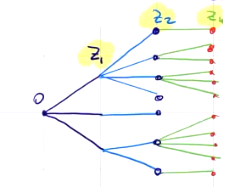
\includegraphics[width=0.5\linewidth]{screenshot015}
			\caption{I don't even know anymore.}
			\label{fig:screenshot015}
		\end{figure}
		The offsprings have a distribution $\{p_{k}\}$. The mean number of offsprings per individual is $m=\sum kp_{k}$. Consider the i.i.id \rv s $\{Z^{(n)}(i),n\geq 0\}$ describing the number of children of the $i$-th individual of generation $n$. Define 
		\begin{equation*}
			Z_{n+1}=\begin{cases}
				Z^{(n)}(1)+Z^{n}(2)+\ldots+Z^{(n)}(Z_{n})&\text{if }Z_{n}\neq 0\\
				0&\text{if }Z_{n}=0
			\end{cases}
		\end{equation*}
		We immediately realize that this is a Markov process because every generation's number of children can be entirely derived from the previous generation's law or reproduction. I don't need to know whose child the individual is. So $Z_{n}$ (number of individual of the $n$-th generation) gives rise to a Markov chain. 
		\begin{equation*}
			\sum_{j=0}^{\infty}p_{ij}j=m\cdot i
		\end{equation*}
		Is the equation that tells us the complete number of individuals. Now consider $Pf=mf$ with $f(j)=j$. So we have $Pj=mi$ where $m$ plays the role of $\lambda$. The process $\{\frac{Z_{n}}{m^{n}},\sigma(Z^{(0)},\ldots,Z^{(n)})\}$ is a martingale. 
	\end{example}
	\subsubsection*{Poisson martingale}
	Consider $\R_{+}$ as our index set. $\F$ is our filtration and we consider the counting process $N={(N_{t})}_{t\geq 0}$ (it counts the number of events up to time $t$). It has unit jumps and any path starts from 0 ($N_0(\omega)=0$), is increasing and right continuous.
	\begin{definition}
		The counting process $N$ is said to be a \emph{Poisson process} with rate $\lambda$ with respect to $\F$ if it is adapted to $\F$ and
		\[\ev[f(N_{t+s}-N_s)|\F_s]=\sum_{k=0}^{\infty}e^{-\lambda t}\frac{(\lambda t)^{k}}{k!}f(k)\qquad\every s,t\in\R_+,\every\text{positive }f\mapsto\N.\]
	\end{definition}
	\begin{theorem}
		Let $N$ be a counting process. It is a Poisson process with rate $\lambda$ with respect to $\F$ \ifonly{}:
		\begin{equation*}
			M_{t}=N_{t}-\lambda t
		\end{equation*}
		is a $\F$-martingale.
	\end{theorem}
	We only prove that $M_t$ is a martingale if $N_{t}$ is Poisson.
	\begin{fancyproof}
		We know that 
		\begin{align*}
			\ev[M_{t}|\F_{s}]&=\ev[M_{t}-M_{s}+M_{s}|\F_{s}]\\
			&=\ev[M_{t}-M_{s}|\F_{s}]+M_{s}\\
			&=\ev[M_{t}-M_{s}]+M_{s}\\
			&=\ev[N_{t}-N_{s}+\lambda t+\lambda s]+M_{s}\\
			&=\underbrace{\ev[N_{t}-N_{s}]}_{\cancel{\lambda (t-s)}}-\cancel{\lambda (t-s)}+M_{s}\\
			&=M_{s}
		\end{align*}
	\end{fancyproof}
	We may use the Doob's decomposition theorem to get $N_{t}=M_{t}+\lambda t$ where $\lambda t$ is our predictable process. So the same result can be achieved from two different viewpoints.
	\subsection{Integration in discrete time}
	Let us consider two real-valued processes $M={(M_{n})}_{n}$ and $F={(F_{n})}_{n}$ and let us define
	\[X_{n}=F_0M_{0}+(M_1-M_0)F_1+\ldots+(M_{n}-M_{n-1})F_n.\]
	We say that $\{X_{n}\}$ is the integral of $F$ with respect to $M$ and we write
	\[X_{n}=\int F \dif M\]
	where $\dif M$ is a random signed measure. Remember the Lebesgue-Stieltjes integral? Me neither, but as long as $M$ has bounded variation this is a Lebesgue-Stieltjes integral.
	\begin{flushright}
		\begin{tikzpicture}
			\calloutquote[width=4cm,position={(1,-1)},fill=Turquoise4!30,rounded corners]{Yeah no wait hold your fucking horses.}
		\end{tikzpicture}\hspace*{2.5cm}
	\end{flushright}
	\hspace{2cm}
	\begin{tikzpicture}
		\calloutquote[width=3cm,position={(-1,-1)},fill=DodgerBlue4,rounded corners]{\color{white}What's up now?}
	\end{tikzpicture}
	\begin{flushright}
		\begin{tikzpicture}
			\calloutquote[width=5cm,position={(1,-1)},fill=Turquoise4!30,rounded corners]{First of all how is that shit an integral?? And what the fuck is a Lebesgue-Stieltjes integral?}
		\end{tikzpicture}\hspace*{2.5cm}
	\end{flushright}
	\hspace{2cm}
	\begin{tikzpicture}
		\calloutquote[width=5cm,position={(-1,-1)},fill=DodgerBlue4,rounded corners]{\color{white}I should have NEVER let you enroll in this master.}
	\end{tikzpicture}
	\begin{flushright}
		\begin{tikzpicture}
			\calloutquote[width=5cm,position={(1,-1)},fill=Turquoise4!30,rounded corners]{Professor Lods, I will exact my revenge on Università di Torino very soon.}
		\end{tikzpicture}\hspace*{2.5cm}
	\end{flushright}
	Okay okay. So a little explanation is due since I actually never saw a Stieltjes integral. Too busy doing things, y'know. Things like, for example, sex. Heh. Yeah. Sex. 
	\begin{revise}
		Oookay so very shortly: a Riemann-Stieltjes integral is a generalization of our dear old Riemann integral. It is notated as
		\begin{equation*}
			\int_{a}^{b}f(x)dg(x).
		\end{equation*}
		Actually this is not too different from the concept of the Lebesgue integral. Basically is about partitioning the interval $(a,b)$ and then summing for every partition (that is, for each $i$) each value of $f(x_i)$ multiplied for $[g(x_i)-g(x_{i-1})]$. Just take the limit for the partition to be infinitely small and voilà, le integràl c'est servie (I don't know French). El integral està servido (I know a little bit of Spanish). Omnibus integral paratum est ut facile intellegatur (I actually know Latin really well. Useless skills are my strength).\par
		Anyway what's important is: \textit{we take the function $f(x)$ and use it to calculate how much the variation of $g(x)$ impacts on the total sum}. And if $g(x)=x$, well... We have our cute little Riemann integral!
	\end{revise}
	Yeah after this smug declaration of sterile knowledge we are maybe ready to better understand how the discrete time integral is, well, an integral. Our function $g(x)$ is $M$ so we consider the variation of $M$; since we are working in discrete time we will never reach a partition so fine it can be called continuous. So it's like... a \textit{diet} Riemann-Stieltjes integral.
	\begin{theorem}
		Consider $F$ bounded and predictable. Then if $M$ is a martingale then $X$ is a martingale; If $M$ is a sub(super)-martingale then $X$ is a sub(super)-martingale.
	\end{theorem}
	This means that... \emph{we can't beat the system!}
	\begin{flushright}
		\begin{tikzpicture}
			\calloutquote[width=4cm,position={(1,-1)},fill=Turquoise4!30,rounded corners]{I can beat something else though.}
		\end{tikzpicture}\hspace*{2.5cm}
	\end{flushright}
	\begin{example}
		Consider $M_{n}$ as the price of a share at time $n$ and $F_{n}$ as the number of shares owned during $(n-1,n]$. Our profit will be 
		\[(M_{n}-M_{n=1})F_{n}\]
		and our total profit $X_{n}$ gained during $(0,n]$ will be:
		\[X_{n}=X_{0}+\underbrace{\sum_{k=1}^{n}(M_{k}-M_{k-1})F_{k}}_{\mathclap{\text{discrete time integral}}}\]
		$F_{n}$ is based on the knowledge in $n-1$ so it is predictable. The process $M_{n}$ should be a martingale (otherwise if it is a sub/super-martingale everyone/no one will buy). So the total profit will also be a martingale! We can only choose our buying politics $F_{k}$, but there is no way to select a politics that will change a martingale in a super-martingale or sub-martingale.
	\end{example}
	Clearly this works in mean! 
	\begin{fancyproof}
		\begin{enumerate}
			\item	We have $M$ being a martingale and $F_0,F_1,\ldots,F_n\in\F_{n}$ as well as $M_0,M_1,\ldots,M_{n}\in\F_n$. Therefore $X_{n}\in\F_{n}$ and $X$ is adapted to $\F$.
			\item We need to check whether the discrete time integral is a martingale. We know by hypothesis that $F$ is bounded, so $F<b$ for some $b$. This implies
			\begin{equation*}
				|X_{n}|<b(|M_{0}|+|M_1+M_0|+\ldots+|M_n-M_{n-1}|)
			\end{equation*}
			Since $M$ is a martingale and it is integrable, we get that $X_n$ is bounded and integrable.
			\item Consider
			\begin{equation*}
				\ev[X_{n+1}-X_{n}|\F]=\ev[F_{n+1}(M_{n+1}-M_{n})|\F_n]
			\end{equation*}
			since all the terms cancel out and only the last ones survive. But $F_{n+1}\in\F_{n}$ so we can take it out of the expectation:
			\[F_{n}\underbrace{\ev[M_{n+1}-M_{n}|\F_{n}]}_{=0}=0.\]
		\end{enumerate}
	\end{fancyproof}
	We know that using a policy that it is predictable it is impossible to beat the system. Finance bros try to overcome this possibility using stopping times. If my policy is not only based on a predictable process but I add the randomness of the time in which I decide to sell or buy can I break the curse of martingales and make shareholders want to suck my dick? Well, it depends.
	\subsection{Stopped martingales and Doob's stopping theorem}
	\begin{definition}
		Define $M={(M_{n})}_{n\in\N}$ as a process and let $T$ be a random time with values on $\overline{\N}$. The process
		\[X_{n}(\omega)=M_{n\wedge T}(\omega)=\begin{cases}
			M_{n}(\omega)&n<T(\omega)\\
			M_{T}(\omega)&n>T(\omega)
		\end{cases}\]
		(where $n\wedge T$ is a truncated random time) is called \emph{$M$ stopped at $T$}.
	\end{definition}
	As a consequence $X$ is exactly the discrete time integral if $F=\indi_{[0,T]}$:
	\begin{equation*}
		X_{n}=\underbracket[0.6pt]{M_0F_0}_{0}+(M_{1}+M_{0})\indi_{[0,T]}(1)+\ldots+(M_{n}-M_{n-1})\indi_{[0,T]}(n).
	\end{equation*}
	The indicators only select the current time interval. If this is the case we can observe that $F_{[0,T]}$ is bounded, positive and predictable. Hence if $M$ is a martingale the theorem applies with this special choice of $M$ and we can write the result as a different theorem:
	\begin{theorem}
		Let $T$ be a stopping time and let $X$ be the process $M$ stopped at $T$. If $M$ is a martingale then so is $X$ (the same holds for sub-martingales and super-martingales).
	\end{theorem}
	So we cannot determine a policy based on stopping times that can change the nature of our martingale. In the remote case in which you are interested in this you can read Williams - Introduction to martingales. \\
	A further theorem about this is \emph{Doob's stopping theorem}. For a martingale we know
	\[\ev[X_{t}-X_{s}|\F_{s}]=0.\]
	The question is: is this true also if $s$ and $t$ are substituted by stopping times $S,T,S\leq T$?
	\begin{theorem}
		Let $M$ be adapted to $\F$. Then the following are equivalent:
		\begin{enumerate}[\circnum]
			\item $M$ is a submartingale;
			\item for every bounded stopping time $S\leq T$ the \rv s $M_{S}$ and $M_{T}$ are integrable and 
			\[\ev[M_{T}-M_{S}|\F_{S}]\geq0;\]
			\item for each pair of bounded stopping times the \rv s $M_{S}$ and $M_{T}$ are integrable and 
			\[\ev[M_{T}-M_{S}]\geq 0.\] 
		\end{enumerate}
	\end{theorem}
	\begin{remark}
		If $M$ is a martingale the theorem can be read in a different way:
		\begin{equation*}
			\ev M_{T}=\ev M_{S}=\ev M_{0}.
		\end{equation*}
		Previously, $\ev M_{n}=\ev M_{n-1}=\ev M_{0}$.
	\end{remark}
	\begin{fancyproof}
		To prove the theorem we need to show that from condition 1 follows 2 from which follows 3 from which follows 1.
		\begin{enumerate}
			\item[$1\to 2$] by hypothesis $M$ is a sub-martingale and our thesis is that if $S(\omega)<T(\omega)<n$ (because we asked for bounded times) then:
			\begin{enumerate}
				\item $M_{S}$ and $M_{T}$ are integrable;
				\item $\ev[M_{T}-M_{S}|\F_{S}]\geq0$.
			\end{enumerate}
			We know that $S$ and $T$ are bounded by $n$. Let $V$ be a positive bounded \rv{} and define $F=V\indi_{(S,T]}$ and use it in the discrete time integral:
			\[X_{n}=\underbrace{M_0F_0}_{X_0}+(M_1-M_0)\underbrace{F_1}_{\mathclap{V\indi_{\{1\in(S,T]\}}}}+\ldots+(M_{n}-M_{n-1})F_{n}\]
			So we have 
			\[X_{n}-X_{0}=V(M_{T}-M_{S})\]
			So $X_{n}$ is a sub-martingale. Take $V=1$ and $S=0$: now we have
			\begin{equation*}
				\begin{array}{c c c l}
					X_{n}&-&X_{0}&=M_{T}\\
					\downarrow&&\downarrow&\\
					\text{int.}&&\text{int.}&\implies M_{T}\text{ is integrable}.
				\end{array}
			\end{equation*}
			Now take $V=1$ and $T=n$ so that we get
			\begin{equation*}
				\begin{array}{c c c c l}
					X_{n}&-&X_{0}&=M_{n}&-M_{S}\\
					\downarrow&&\downarrow&\downarrow&\\
					\text{int.}&&\text{int.}&\text{int.}&\implies M_{S}\text{ is integrable}.
				\end{array}
			\end{equation*}
			We recall that $V\in\F_S$ and we use the defining property for $\ev(\cdot|\F_S)$. So we can write
			\begin{align*}
				\ev V\ev(M_{T}-M_{S}|\F_{S})&\underset{\mathclap{\text{def. prop.}}}{=}\ev V(M_{T}-M_{S})\\
				&\underset{\mathllap{\text{discr. time int.}}}{=}\ev[X_{n}-X_{0}]\\
				&\underset{\mathllap{\text{proved above}}}{\geq}0
			\end{align*}
			and this is true $\every V>0,V<b,V\in\F_{s}$. Hence
			\begin{equation*}
				\ev(M_{T}-M_{S}|\F_{S})\geq 0
			\end{equation*}
			So $1\to2$.
			\item[$2\to3$] We can use the tower rule. Take the expectation of point 2:
			\[\ev[\ev(M_{T}-M_{S}|\F_{S})]=\ev[M_{T}-M_{S}]\geq0.\]
			\item[$3\to1$] Let $3$ hold, so that $\ev[M_{T}-M_{S}]\geq0$. Choose $T=n$ and $S=0$. Then
			$M_{n}$ is integrable. Move to adaptness: this holds by hypothesis. Move to the martingale inequality:
			\begin{equation*}
				\ev[M_{n}-M_{m}|\F_{m}]\geq0.
			\end{equation*}
			Note that this is equivalent to prove 
			\begin{equation*}
				\ev\indi_H\ev[M_{n}-M_{m}|\F_{m}]\geq0\qquad H\in\F_{m},0\leq m\leq n.
			\end{equation*}
			Fix $H,m,n$ and define
			\begin{equation*}
				S(\omega)=m\qquad T(\omega)=n\indi_H(\omega)+m\indi_{\{\Omega\setminus H\}}(\omega)
			\end{equation*}
			The indicators are non-zero in complementary instances. Notice that:
			\begin{enumerate}
				\item $S$ is a fixed time so it is a stopping time;
				\item $S\leq T\leq n$ by definition of $S$ and $T$ because the indicators are non-zero in complementary instances;
				\item $T\geq S$ is a foretold time by $S=m$;
				\item $H\in\F_{S}$ by definition.
			\end{enumerate}
			So we can write $M_{T}-M_{S}=\indi_H(M_{n}-M_{m})$ where $M_{T}-M_{S}\geq0$ by hypothesis. This means that we have 
			\begin{equation*}
				\underbrace{\ev[\indi_{H}\ev(M_{n}-M_{m}|\F_{m})]}_{\ev[M_{n}-M_{m}|\F_{m}]\geq0}\geq0
			\end{equation*}
		\end{enumerate}
	\end{fancyproof}
	\subsection{Oscillations}
	We will talk about oscillations in a strip $(a.b)$ during a time interval. Consider an adapted process $M$ and two real numbers $a<b\in\R$. We want to set a level $a$ and a level $b$. First, by convention, fix $T_0=-1$. Then define:
	\[\begin{array}{l}
		S_{k}:=\inf\{n>T_{k-1}:M_{n}\leq a\}\\
		T_{l}:=\inf\{n>S_{k}:M_{n}\geq b\}.
	\end{array}\]
	So it is the first time in which the process crosses the threshold $a$ or $b$ after having crossed the other threshold.
	\begin{figure}[h]
		\centering
		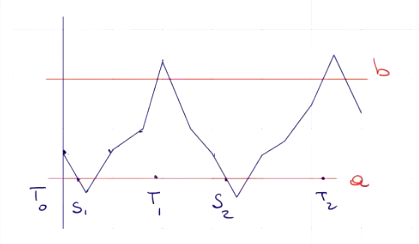
\includegraphics[width=0.62\linewidth]{screenshot016}
		\caption{Up and downs. Just like my consumption of cocaine and my mood respectively on an average tuesday evening.}
		\label{fig:screenshot016}
	\end{figure}
	We call $S_{k}$\emph{ downcorssing time} while we call $T_{k}$ \emph{upcrossing time}. \\
	Now consider the sequence $(T_0,S_1,T_1,S_2,T_2,\ldots)$. It is an increasing sequence of stopping times. If we want to focus on the number of oscillations we may count how many times we go from an upcrossing to a downcrossing time (or vice-versa). Say we want to count the upcrossing. We can define a quantity
	\begin{equation*}
		U_{n}(a,b)=\sum_{k=1}^{\infty}\indi_{(0,n]}(T_{k})
	\end{equation*}
	which of course is a counting process.
	\begin{example}
		We are still with our financebros. Suppose that $(M_{n})$ is the price of an asset at time $n$. We want to buy when the price is below $a$ at time $S_i$ and sell when it is above $b$ at time $T_i$. In $(0,n]$ we have $U_{n}(a,b)$ cycles of buying and selling so our strategy could consists in holding a number $F_{n}$ of shares during period $(m-1,m]$. This means introducing
		\[F_{m}=\sum_{k=1}^{\infty}\indi_{(S_{k},T_{k}]}\]
		with $F_{0}=0$. We can thus trace the evolution of our capital with the discrete-time integral:
		\[X=\int F\dif M\]
		And the profit during $(0,n]$will be $X-X_{0}$.\\
		The profit is at least
		\begin{equation*}
			(b-a)U_{n}(a,b).
		\end{equation*}
	\end{example}
	\begin{proposition}
		If $M$ is a sub-martingale with respect to its natural filtration then 
		\begin{equation*}
			(b-a)\ev U_{n}(a,b)\leq\ev\left[(M_{n}-a)^{+}-(M_{0}-a)^{+}\right].
		\end{equation*}
	\end{proposition}
	We wanted to find a bound for our profit, but our profit is a stochastic quantity: so it's only natural to think about the expectation to give a bound to the number of expected up/downcrossing.\\
	Observe that the number of upcrossings does not depend on the value of $T_0$ that we fix.
	\begin{fancyproof}
		Choose $a=0$. Consider hence the process $(M-a)^{+}$ that is sub-martingale (if $M$ is a sub-martingale). Take $M\geq 0$ and let 
		\begin{equation*}
			F_{n}-\sum_{k=1}^{\infty}\indi_{(S_{k},T_{k}]}(n)
		\end{equation*}
		and consider 
		\begin{equation*}
			X=\int F\dif M
		\end{equation*}
		like in our example. We know that $F$ is predictable since by definition $F_{k+1}\in\F_{k}$. Consider the expectation of the increment
		\begin{equation*}
			\ev[X_{k+1}-X_{k}|\F_{k}]=\ev\left[F_{k+1}(M_{k+1}-M_{k})|\F_{k}\right].
		\end{equation*}
		But since $F_{k+1}$ is predictable we can take it out the expectation:
		\begin{equation*}
			F_{k+1}\ev\left[M_{k+1}-M_{k}|\F_{k}\right].
		\end{equation*}
		But since $F_{k+1}$ is an indicator we know it is $\leq1$:
		\begin{equation*}
			\ev[X_{k+1}-X_{k}|\F_{k}]\leq\ev\left[M_{k+1}-M_{k}|\F_{k}\right].
		\end{equation*}
		Now take the expectation of both sides:
		\begin{equation*}
			\ev[X_{k+1}-X_{k}]\leq\ev\left[M_{k+1}-M_{k}\right].
		\end{equation*}
		If we sum these inequalities over $k$ we get:
		\begin{equation*}
			\ev\left[X_{n}-X_{0}\right]\leq\ev\left[M_{n}-M_{0}\right].
		\end{equation*}
		So we now get that
		\begin{equation*}
			bU_{n}(a,n)\leq\ev\left[X_{n}-X_{0}\right]\leq\ev\left[M_{n}-M_{0}\right]
		\end{equation*}
		but given that $a=0$ we get that
		\begin{equation*}
			bU_{n}(0,b)\leq\ev[M_{n}-M_{0}].
		\end{equation*}
		Clearly we have to take the positive part.
	\end{fancyproof}
	This characterizes our martingale and its boundedness. The number of oscillations of a sub-martingale is bounded! The next question is: can we say anything about the behaviour of maximum/minimum of a martingale or sub-martingale? 
	\begin{remark}
		Consider a sequence $\{X_{n}\}$ of independent \rv s with $\ev X_{n}=0,S_n=\sum X_{i}$. We proved that
		\begin{equation*}
			a^{2}\pr(\max_{k\leq n}|S_{k}|>a)\leq\var S_{n}
		\end{equation*}
		and we called this \emph{Kolmogorov's inequality}.
	\end{remark}
	What we are doing here is considering a random walk whose jumps have 0 mean. We wonder wether it is above the level $a$ as seen in figure \ref{fig:screenshot017}.
	\begin{figure}[h]
		\centering
		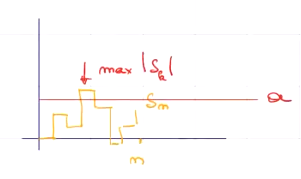
\includegraphics[width=0.6\linewidth]{screenshot017}
		\caption{The maximum of the random walk.}
		\label{fig:screenshot017}
	\end{figure}
	About this, we know that $\{S_{n}\}$ is a $\F$-martingale but in proving the Kolmogorov's inequaility we never talked about the martingale property! We could improve this inequality using the \emph{Doob's martingale inequality}. The problem is that we can prove very general inequalities that hold true for any \rv s but specifying more characteristic we can obtain stricter bounds. In this framework let's define 
	\begin{equation*}
		\begin{array}{l}
			M^{\star}_{n}=\max_{k\leq n}M_{k}\\
			m^{\star}_{n}=\min_{k\leq n}M_{k}\\
		\end{array}
	\end{equation*}
	as current maximum and current minimum of $M$.
	\begin{theorem}
		Take $M$ as a sub-martingale. For $b>0$ it holds:
		\begin{enumerate}
			\item $b\pr(M^{\star}_{n}\geq b)\leq\ev\left[M_{n}\indi_{\{M_{n}^{\star}\geq b\}}\right]\leq\ev\left[M_{n}^{+}\right]$;
			\item $b\pr(m^{\star}_{n}\leq-b)\leq-\ev M_{0}+\ev\left[M_{n}\indi_{\{m_{n}^{\star}\geq b\}}\right]\leq\ev M_{n}^{+}-\ev M_{0}$.
		\end{enumerate}
	\end{theorem}
	So we can further bound the result looking into the property of $M_{n}$.
	\begin{example}
		Prof. Sacerdote fucked up so we now need to define the brownian motion (or Weiner process).
		\begin{definition}
			A real-valued stochastic process $B={(B_{t})}_{t\geq0}$ is called \emph{brownian motion} if:
			\begin{enumerate}
				\item the index set is $\R^{+}$;
				\item $B_{0}(\omega)=0$ for almost all $\omega$;
				\item $B_{t_{n}}-B_{t_{n-1}},\ldots,B_{t_{1}}-B_{t_{0}}$ are independent for $\every 0=t_{0}<t_1<\ldots<t_n<\infty$;
				\item $B_{t}-B_{s}\sim B_{t+b}-B_{s+b}$ for every $0\leq s<t<\infty\quad\every n>- s$;
				\item $B_{t}-B_{s}\sim N(0,t-s)$;
				\item $t\mapsto B_{t}(\omega)$ are continuous for every $\omega$.
			\end{enumerate}
		\end{definition}
		The brownian motion is in itself a martingale, but there is a class of martingales strictly related to it:
		\begin{equation*}
			M_{t}=\exp\left\{\lambda B_{t}-\frac{1}{2}\lambda^{2}t\right\},\qquad t\in\R^{+}.
		\end{equation*}
		Now we can get to the actual example: if $B$ is a brownian motion, we have 
		\begin{equation*}
			\pr(\sup_{0\leq t\leq\theta}B_{t}\geq b)\leq\exp\left\{-\frac{b^{2}}{s\theta}\right\}.
		\end{equation*}
		The sample paths of brownian motions are extremely irregular. We are asking with which probability the max of our process will be over $b$ at time $\theta$.
		\begin{figure}[H]
			\centering
			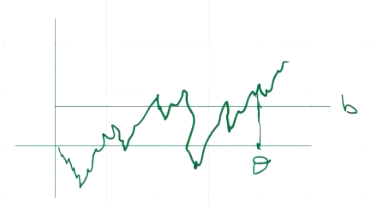
\includegraphics[width=0.6\linewidth]{screenshot018}
			\caption{Check out Autechre. A staple in electronic experimental music.}
			\label{fig:screenshot018}
		\end{figure}
		I am basically asking if the maximum attained is above or below $b$.
		How can we use the Doob's inequality?
		\begin{fancyproof}
			Consider
			\begin{equation*}
				\pr(\sup B_{t}\geq b)=\pr(\sup e^{\lambda B_{t}}\geq e^{\lambda b})
			\end{equation*}
			and using Doob's inequality
			\begin{align*}
				\pr(\sup B_{t}\geq b)&=\pr(\sup e^{\lambda B_{t}}\geq e^{\lambda b})\\
				&\leq \frac{\overbrace{\ev\left[e^{\lambda B_{\theta}-\frac{\lambda^{2}}{2}\theta}\right]}^{\text{martingale}}}{e^{\lambda b}e^{-\frac{\lambda^{2}}{2}\theta}}\\
				&=e^{-\lambda b+\frac{\lambda^{2}}{2}\theta}\qquad\every\lambda>0
			\end{align*}
		\end{fancyproof}
	\end{example}
	Now we have to prove Doob's inequality.
	\begin{fancyproof}
		We introduce 2 stopping times: 
		\begin{equation*}
			\begin{array}{l l}
				T&=\inf\{n\geq0:M_{n}\geq b\}\\
				S&=\inf\{n\geq0:M_{n}\leq-b\}.
			\end{array}
		\end{equation*}
		\begin{figure}[H]
			\centering
			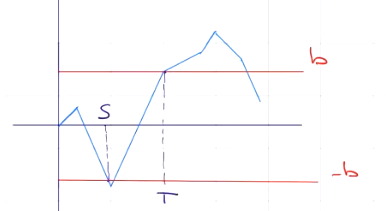
\includegraphics[width=0.6\linewidth]{screenshot019}
			\caption{Also Aphex Twin. Really, Autechre and Aphex Twin are probably the best example of the boom of experimentation in popular electronic music between 1995 and 2005.}
			\label{fig:screenshot019}
		\end{figure}
		Consider the current maximum and minimum above the level $b$:
		\begin{equation*}
			\{M^{\star}_{n}\geq b\}=\{T\leq n\}\qquad	\{m^{\star}_{n}<-b\}=\{S\leq n\}.
		\end{equation*}
		Fix $b$ and $n$. When $\{T\leq n\}$ we have
		\begin{align*}
			M_{T\wedge n}=M_{T}\geq b.
		\end{align*}
		Multiply by $\indi_{\{T\leq n\}}$:
		\begin{equation*}
			b\indi_{\{T\leq n\}}\leq M_{T\wedge m}\indi_{\{T\leq n\}}.
		\end{equation*}
		Using Doob's stopping theorem we know that 
		\begin{equation*}
			\ev\left[M_{T}-M_{S}|\F_{S}\right]\geq0
		\end{equation*}
		and using $S=T\wedge n$ and $T=n$ we obtain
		\begin{equation*}
			\ev\left[M_{n}|\F_{T\wedge n}\right]>M_{T\wedge n}.
		\end{equation*}
		So summing it all up:
		\begin{align*}
			b\indi_{\{T\leq n\}}&\leq M_{T\wedge m}\indi_{\{T\leq n\}}\\
			&\leq\indi_{\{T\leq n\}}\ev\left[M_{n}|\F_{T\wedge n}\right]\\
			&\ev\left[M_{n}\indi_{\{T\leq n\}}|\F_{T\wedge n}\right].
		\end{align*}
		Now take the expectation:
		\begin{align*}
			b\pr(T\leq n)&=b\pr(M^{\star}_{n}\geq b)\\
			&\leq\underbrace{\ev\left[M_{n}\indi_{\{T\leq n\}}\right]}_{\mathclap{\ev\left[M_{n}\indi_{\{M_{n}^{\star}\geq b\}}\right]}}\\
			&\leq\ev(M^{+}_{n}).
		\end{align*}
		For the minimum we work on $\{S\leq n\}$ and we get 
		\begin{align*}
			M_{S\wedge n}&=M_{S}\indi_{\{S\leq n\}}+M_{S}\indi_{\{S>n\}}\\
			&\leq-b\indi_{\{S\leq n\}}+M_{n}\indi_{S\geq n}.
		\end{align*}
		Now take the expectation:
		\begin{equation*}
			\ev M_{S\wedge n}\leq-b\pr(m^{\star}_{n}\leq-b)+\ev\left[M_{n}\indi_{\{S>n\}}\right].
		\end{equation*}
		So that we get
		\begin{equation*}
			\pr(m^{\star}_{n}\leq-b)\leq-\ev M_{S\wedge n}+\ev[M_{n}\indi_{\{S>n\}}].
		\end{equation*}
		Now use Doob's stopping theorem with $T=0$ and $S=S\wedge n$ so that $\ev M_{0}\leq\ev M_{\{S\wedge n\}}$. This gets us our result:
		\begin{align*}
			b\pr(m^{\star}_{n}-b)&\leq-\ev M_{0}+\ev\left[M_{n}\indi_{\{m_{n}^{\star}\}}\right]\\
			&\leq\ev M^{+}_{n}-\ev M_{0}.
		\end{align*}
	\end{fancyproof}
	\begin{remark}
		If $M$ is a martingale then $|M|^{p}$ is a sub-martingale for $p\geq1$. If $M_{n}\in\lp\every n$ we can apply Doob's inequality.
	\end{remark}
	\begin{corollary}
		If $M$ is martingale in $\lp$ for some $p\geq 1$ then for $b>0$ we have that
		\begin{equation*}
			b^{p}\pr(\max_{k\leq n}|M_{k}|>b)\leq\ev|M_{n}|^{p}.
		\end{equation*}
	\end{corollary}
	There are also other bounds:
	\begin{itemize}
		\item $b\pr(\max_{k\leq n}|M_{k}>b)\leq 2\ev M_{n}^{+}-3M_{0}$;
		\item \emph{Doob's norm inequality}: if $M$ is a martingale in $\lp,p\geq 1$ and $q$ is the exponent conjugate to $p$ ($\frac{1}{p}+\frac{1}{q}=1$) then
		\begin{equation*}
			\ev\max_{  k\leq n}|M_{k}|^{p}\leq q^{p}\ev|M_{n}|^{p}.
		\end{equation*}
		\item  Consider $L^{2}$-bounded martingales characterized by final coordinate $X$ with $\var X=\sigma^{2}$ (that is I am fixing the variance of the last value I consider). We want to assess the variability of this process.
		\begin{theorem}
			\emph{Dubin \& Schwartz 1998}: it holds
			\begin{enumerate}
				\item $\ev\left[\max_{0\leq T\leq t}M_{T}\right]\leq\sigma$;
				\item $\ev\left[\max_{0\leq T\leq t}|M_{T}|\right]\leq\sigma\sqrt{2}$.
			\end{enumerate}
			Moreover, there exist suitable martingales for which this bound is attained and is scrict.
		\end{theorem}
	\end{itemize}
	\subsection{Limit of sequences of \rv s}
	Consider a sequence of \rv s $\{X_{n}\}$ with independence between the \rv. Then we know that if $\lim X_{n}$ exists then the limit is a constant. Why?
	\begin{remark}
		If the $\lim_{n}X_{n}$ exists than it belongs to the tail \sa{} $\tau$. Since the \rv s are independent then we can apply the 0-1 Kolmogorov law, so the probability that the \rv{} is infinity is either 0 or 1 but if this is the case then it must be a constant.
	\end{remark}
	This is about the behavior in the limits of a sequence of \rv s with independence between $\{X_{n}\}$. Then if the limit exists it is a constant, since $\lim_{n}X_{n}$ belongs to the tail \sa{} of the sequence. Independency between \rv s tells us that we can apply Kolmogorov's 0-1 law to say that $\pr(\lim_{n}X_{n}=\infty)$ is either 0 or 1... but if we somehow know that the limit exists then it can't be $\infty$ so its probability of being $\infty$ is 0 and therefore it is a constant almost surely! This is cool because it tells us that the limit is either infinite or finite.
	If $\{X_{n}\}$ is a submartingale consider the limit 
	\begin{equation*}
		\lim_{n\to\infty}X_{n}=X_{\infty}
	\end{equation*}
	What the fuck? What is this object? Consider the case in which $\T=\N$. We know that the expected value $\{\ev X_{n}\}$ is an increasing sequence if the process is a sub-martingale. 
	We have our first theorem about convergence:
	\begin{theorem}
		Let $X$ be a sub-martingale. If (and note that is a sufficient condition)
		\begin{equation*}
			\sup_{n}\ev X_{n}^{+}<\infty
		\end{equation*}
		Then
		\begin{enumerate}
			\item $\{X_{n}\}$ converges $\as$;
			\item $\{X_{n}\}$ converges to an integrable \rv.
		\end{enumerate}
	\end{theorem}
	Before proving think about it. \begin{enumerate}
		\item	The condition of this theorem requires that $X^{+}$ is in $L^{1}$ and is bounded. If $X$ is a sub-martingale then also $X^{+}$ is a sub-martingale... But this means that $\ev X^{+}_{n}$ is an increasing sequence. Our condition gives a bound to the increase of this sequence! But this means that I am trying to avoid the divergence of the expected value (which means: trying to control the rate of our martingale). 
		\item Now think about a negative sub-martingale: this would verify the condition so there is no problem about it.
		\item Now think about a positive super-martingale: it is only a negative sub-martingale with another sign so it converges.
		\item Consider now a positive or bounded martingale or a negative martingale. All of these cases converge. 
		\item $\sup\ev X_{n}^{+}<\infty\iff\sup\ev|X_{n}|\leq\infty$. Let $\{X_{n}\}$ be a sub-martingale such that
		\begin{equation*}
			\ev X_{n}>\ev X_{0}\qquad\every n.
		\end{equation*}
		But now \begin{equation*}
			\ev|X_{n}|=\ev X_{n}^{+}-\ev X_{n}^{-}=\ev X_{n}^{+}+\ev_{n}^{+}-\ev X_{n}
		\end{equation*}
		So
		\begin{align*}
			\ev X_{n}^{+}&\leq\ev|X_{n}|=2\ev X_{n}^{+}-\ev X_{n}\\
			&\leq 2\underbrace{\ev X_{n}^{+}}_{<\infty}-\ev X_{0}\leq\infty
		\end{align*}
		So $\ev|X_{n}|\leq\infty$.
	\end{enumerate}
	\begin{fancyproof}
		We prove the theorem by contradiction. Pick an outcome $\omega$ and suppose that $\{X_{n}(\omega)\}$ is a numerical sequence that has not a limit. But if it doesn't have a limit, then 
		\[\exists\inf\lim\neq\sup\lim\qquad\inf\lim<\sup\lim.\]
		So there exist at least 2 rationals $a<b$ such that
		\begin{equation*}
			\inf\lim<a<b<\sup\lim.
		\end{equation*}
		The sequence $\{X_{n}(\omega)\}$ crosses $(a,b)$ $\infty$ many times. Now take the union over rational $a$ and $b$, $a<b$ of the sets
		\begin{equation*}
			\{U(a,b)=\infty\}
		\end{equation*}
		with $U(a,b)=\lim_{n\to\infty}U_{n}(a,b)$. Our aim is now to show that $U(a,b)\leq\infty$ almost surely to get a contradiction.\\
		Fix $a,b$. We know that $U_{n}(a,b)$ is increasing with $n$. Now consider
		\begin{align*}
			(b-a)\ev U(a,b)&=(b-a)\ev\lim U_{n}(a,b)\\
			&\underset{\mathclap{\text{monotone conv.}}}{=}(b-a)\lim\ev U_{n}(a,b)\\
			&\underset{\mathclap{\text{upcross inequalities}}}{\leq}\sup\ev(X_n-a)^{+}\\
			&\leq \sup\ev X_{n}^{+}+|a|.
		\end{align*}
		So this means that $\ev U(a,b)<\infty$. But this is a contradiction, so it exists a limit $X_{n}=X_{\infty}\as$.\\
		Now consider the second part of the theorem:
		\begin{align*}
			\ev|X_{\infty}|&=\ev\lim\inf|X_{n}|\\
			&\underset{\mathclap{\text{Fatou's lemma}}}{\leq}\lim\inf\ev|X_{n}|\\
			&\leq 2\sup\ev X_{n}^{+}-\ev X_{0}\leq\infty
		\end{align*}
		so the limit is integrable.
	\end{fancyproof}
	Here everything is related to integrability conditions but this is a sufficient condition. What if we want a sufficient and necessary condition? Well, consider $\sup_n\ev X_{n}^{+}\leq\infty$. We want to control the tail uniformly not only on the tail but on the whole process.
	\begin{figure}[h]
		\centering
		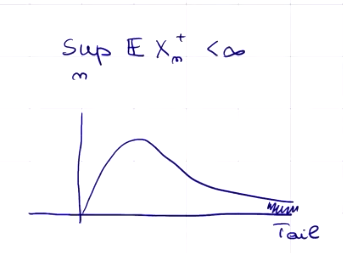
\includegraphics[width=0.6\linewidth]{screenshot020}
		\caption{It's astonishing how much a bad teacher can have you hate a subject.}
		\label{fig:screenshot020}
	\end{figure}
	We recall that we already introduced a strong condition for uniform integrability. w
	We will need:
	\begin{enumerate}
		\item a collection $\mathcal{K}$ of real \rv s is said to be uniformly integrable if 
		\begin{equation*}
			k(b)=\sup_{X\in\mathcal{K}}\ev|X|\indi_{\{X>b\}}\xrightarrow[b\to\infty]{}0.
		\end{equation*}
		\item If $\mathcal{K}$ is dominated by an integrable \rv{} $Z$ then it is uniformly integrable.
		\item uniform integrability implies $L^{1}$-boundedness but not the converse.
		\item If $\mathcal{K}$ is $L^{p}$-bounded for some $p>1$ then it is uniformly integrable.
	\end{enumerate}
	\begin{lemma}
		Let $Z$ be an integrable \rv{}. Then
		\begin{equation*}
			\mathcal{K}=\left\{X:X=\ev(Z|\G)\right\}
		\end{equation*}
		for some sub-\sa{} $\G$ of $\HS$ is uniformly integrable.
	\end{lemma}
	\begin{proposition}
		Let $Z$ be an integrable \rv{}. Define 
		\begin{equation*}
			X_{t}=\ev(Z|\F_{t})\qquad t\in\T.
		\end{equation*}
		This means that $\{X_{t}\}$ is a uniformly integrable $\F$-martingale.
	\end{proposition}
	\begin{theorem}
		Let $\{X_{n}\}$ be a sequence of real-valued \rv s. The following are equivalent:
		\begin{enumerate}
			\item it converges in $L^{1}$;
			\item it converges in probability and it is uniformly integrable.
		\end{enumerate}
	\end{theorem}
	We can now prove the theorem about the convergence of sub-martingales.
	\begin{theorem}
		Let $X$ be a sub-martingale. We have that $X$ converges almost surely and in $L^{1}$ \ifonly{} it is uniformly integrable. Moreover, if it is so, setting 
		\begin{equation*}
			X_{\infty}=\lim X_{n}
		\end{equation*}
		extends $X$ to a sub-martingale
		\begin{equation*}
			\xbar={(X_{n})}_{n\in\overline{\N}}.
		\end{equation*}
	\end{theorem}
	We only prove the first part of the theorem.
	\begin{fancyproof}
		\emph{Necessity}. If $X$ converges in $L^{1}$ by the theorem above it is uniformly integrable.\\
		\emph{Sufficiency}. If $X$ is uniformly integral then it is $L^{1}$-bounded for the property above. So our previous theorem holds and the martingale converges almost surely with $X_{\infty}$ integrable. Furthermore, for the property above, it also converges in $L^{1}$.
	\end{fancyproof}
	Is there a way to get a uniformly integrable sub-martingale?
	\begin{theorem}
		A process $M={(M_{n})}_{n\in\N}$ is a uniformly integrable martingale \ifonly{} for some integrable \rv{} $Z$
		\begin{equation}
			M_{n}=\ev\left[Z|\F_{n}\right]\qquad n\in\N.\tag{$\bullet$}\label{AAAA}
		\end{equation}
		If so it converges almost surely and in $L^{1}$ to the integrable \rv
		\begin{equation*}
			M_{\infty}=\ev[Z|\F_{\infty}].
		\end{equation*}
	\end{theorem}
	\begin{corollary}
		For every integrable \rv{} $Z$ we have
		\begin{equation*}
			\ev(Z|\F_{n})\convas\xrightarrow[]{L^{1}}\ev(Z|\F_{\infty}).
		\end{equation*}
	\end{corollary}
	\begin{theorem}
		Let $Z$ be an integrable \rv{} and let 
		\begin{equation*}
			M_{n}=\ev(Z|\F_{n})_{n\in\overline{\N}}.
		\end{equation*}
		For every stopping time $T$ define
		\begin{equation*}
			M_{T}=\ev[Z|\F_{T}]
		\end{equation*}
		and for arbitrary stopping times $S$ and $T$ we get
		\begin{equation*}
			\ev[M_{T}|\F_{S}]=M_{S\wedge T}.
		\end{equation*}
	\end{theorem}
	This lets us rethink Doob's theorem.
	\begin{theorem}
		If $S$ and $T$ are arbitrary stopping times such that $S\leq T$ then
		\begin{equation*}
			\ev[M_{T}|\F_{S}]=M_{S}
		\end{equation*}
		for an uniformly integrable martingale.
	\end{theorem}
	The dominated convergence theorem requires adaptness. 
	\begin{theorem}
		\emph{Hunt's dominated convergence theorem}.\\
		Let $\{X_{n}\}$ be dominated by an integrable \rv{} and suppose that exists
		\begin{equation*}
			X_{\infty}=\lim X_{n}
		\end{equation*}
		So ${(\ev_{n}X_{n})}_{n}$ converges to $\ev X_{\infty}$ almost surely and in $L^{1}$.
	\end{theorem}
	To prove we should use Borel-cantelli somehow.
\end{document}